\documentclass[10pt]{extarticle}
\title{}
\author{}
\date{}
\usepackage[shortlabels]{enumitem}


%paper setup
\usepackage{geometry}
\geometry{letterpaper, portrait, margin=1in}
\usepackage{fancyhdr}
% sans serif font:
\usepackage{cmbright}
%symbols
\usepackage{amsmath}
\usepackage{bigints}
\usepackage{amssymb}
\usepackage{amsthm}
\usepackage{mathtools}
\usepackage{bbm}
\usepackage{bbold}
\usepackage[hidelinks]{hyperref}
\usepackage{gensymb}
\usepackage{multirow,array}
\usepackage{multicol}

\newtheorem*{remark}{Remark}
\usepackage[T1]{fontenc}
\usepackage[utf8]{inputenc}

%chemistry stuff
%\usepackage[version=4]{mhchem}
%\usepackage{chemfig}

%plotting
\usepackage{pgfplots}
\usepackage{tikz}
\usetikzlibrary{cd}
\tikzset{middleweight/.style={pos = 0.5}}
%\tikzset{weight/.style={pos = 0.5, fill = white}}
%\tikzset{lateweight/.style={pos = 0.75, fill = white}}
%\tikzset{earlyweight/.style={pos = 0.25, fill=white}}

%\usepackage{natbib}

%graphics stuff
\usepackage{graphicx}
\graphicspath{ {./images/} }
\usepackage[style=numeric, backend=biber]{biblatex} % Use the numeric style for Vancouver
\addbibresource{the_bibliography.bib}
%code stuff
%when using minted, make sure to add the -shell-escape flag
%you can use lstlisting if you don't want to use minted
%\usepackage{minted}
%\usemintedstyle{pastie}
%\newminted[javacode]{java}{frame=lines,framesep=2mm,linenos=true,fontsize=\footnotesize,tabsize=3,autogobble,}
%\newminted[cppcode]{cpp}{frame=lines,framesep=2mm,linenos=true,fontsize=\footnotesize,tabsize=3,autogobble,}

%\usepackage{listings}
%\usepackage{color}
%\definecolor{dkgreen}{rgb}{0,0.6,0}
%\definecolor{gray}{rgb}{0.5,0.5,0.5}
%\definecolor{mauve}{rgb}{0.58,0,0.82}
%
%\lstset{frame=tb,
%	language=Java,
%	aboveskip=3mm,
%	belowskip=3mm,
%	showstringspaces=false,
%	columns=flexible,
%	basicstyle={\small\ttfamily},
%	numbers=none,
%	numberstyle=\tiny\color{gray},
%	keywordstyle=\color{blue},
%	commentstyle=\color{dkgreen},
%	stringstyle=\color{mauve},
%	breaklines=true,
%	breakatwhitespace=true,
%	tabsize=3
%}
% text + color boxes
\usepackage[most]{tcolorbox}
\tcbuselibrary{breakable}
\tcbuselibrary{skins}
\newtcolorbox{problem}[1]{colback=white,enhanced,title={\small #1},
          attach boxed title to top center=
{yshift=-\tcboxedtitleheight/2},
boxed title style={size=small,colback=black!60!white}, sharp corners, breakable}
%including PDFs
%\usepackage{pdfpages}
\setlength{\parindent}{0pt}
\usepackage{cancel}
\pagestyle{fancy}
\fancyhf{}
\rhead{Avinash Iyer}
\lhead{Algebra II: Class Notes}
\newcommand{\card}{\text{card}}
\newcommand{\ran}{\text{ran}}
\newcommand{\N}{\mathbb{N}}
\newcommand{\Q}{\mathbb{Q}}
\newcommand{\Z}{\mathbb{Z}}
\newcommand{\R}{\mathbb{R}}
\newcommand{\C}{\mathbb{C}}
\setcounter{secnumdepth}{0}
\begin{document}
  \section{Motivation and Introduction}%
  Main purpose of this course is to study Galois theory --- a field that arose in trying to study roots of polynomials.\\

  Consider $f(x) = ax^2 + bx + c$. If we want to find a general, closed-form expression for the roots of the function, we complete the square.
  \begin{align*}
    \text{roots} &= \frac{-b \pm \sqrt{b^2-4ac}}{2a}.
  \end{align*}
  We found these roots by by the coefficients, $\Q$, addition, subtraction, multiplication, division, and square root (raising to the $1/2$ power: see Math 310 notes, Page 104). Naturally, this leads us to ask whether we can do this for cubic polynomials with the same operations. Obviously, we have to change from $1/2$ power to the $1/3$ power, but Cardano showed that it was possible to solve a cubic and quartic equation using these traditional operations and radicals.\\

  Évariste Galois invented his theory to prove there is no such closed formula by radicals for any polynomial of degree $5$ or above.\\

  For example, $x^5 - x + 1$ does not have roots given by radicals.
  \subsection{Example: A Solvable Polynomial}%
  Consider the polynomial $f(x) = x^2 - 2$. We know that the roots of this polynomial are $\pm \sqrt{2}$. From this, we want to create a set $K(f)$ that satisfies the following rules:
  \begin{itemize}
    \item $\Q \subseteq K(f)$.
    \item $K(f)$ must contain the roots of $f$.
    \item $K(f)$ must be closed under the traditional operations: $+,-,\times,/$
    \item $K(f)$ must be the smallest field that satisfies the above three requirements.
  \end{itemize}
  \textbf{Claim:} $K(f) = \Q(\sqrt{2}) = \{a + b\sqrt{2}\mid a,b\in \Q\}$.
  \begin{itemize}
    \item $\Q\subseteq K(f)$, because we can set $b=0$.
    \item $\sqrt{2} = 0 + (1)(\sqrt{2})$, $-\sqrt{2} = 0 + (-1)(\sqrt{2})$
    \item Let $a+b\sqrt{2}$ and $c+d\sqrt{2}$ be elements of $K(f)$. Then,
      \begin{itemize}
        \item $(a+b\sqrt{2})\pm (c+d\sqrt{2}) = (a\pm c) + (b\pm d)\sqrt{2}$
        \item $(a+b\sqrt{2})(c+d\sqrt{2}) = (ac + 2bd) + (ad + bc)\sqrt{2}$
        \item Set $c+d\sqrt{2} \neq 0$
          \begin{align*}
            \frac{a+b\sqrt{2}}{c+d\sqrt{2}} &= \frac{(a+b\sqrt{2})(c-d\sqrt{2})}{c^2-2d^2}\\
                                            &= \frac{1}{c^2-2d^2}\left((ac-2bd) + (bc-ad)\sqrt{2}\right)\\
                                            &= \frac{ac-2bd}{c^2-2d^2} + \frac{bc-ad}{c^2-2d^2}\sqrt{2}
          \end{align*}
      \end{itemize}
    \item $K(f)$ is indeed the smallest set.
      \begin{itemize}
        \item Note that $K(f)$ is a $\Q$-vector space, with basis $\{1,\sqrt{2}\}$. Therefore, $\text{dim}_{\Q} K(f) = 2$. $K(f)$ is known as the ``splitting field'' of $f$.
      \end{itemize}
  \end{itemize}

  We want to consider a bijective function $\varphi: K(f)\rightarrow K(f)$ with the following properties:
  \begin{itemize}
    \item $\varphi(r) = r$ for every $r\in\Q$
    \item $\varphi(x+y) = \varphi(x) + \varphi(y)$
    \item $\varphi(xy) = \varphi(x)\varphi(y)$
  \end{itemize}
  We denote the collection of all such $\varphi$ as $\text{Aut}(K(f)/\Q)$. This is a group under the operation $\circ$ (composition). Specifically, we have
  \begin{align*}
    \varphi(a+b\sqrt{2}) &= \varphi(a) + \varphi(b)\varphi(\sqrt{2})\\
                         &= a + b\varphi(\sqrt{2}).
  \end{align*}
  Notice
  \begin{align*}
    \left(\varphi(\sqrt{2})\right)^2 - 2 &= \varphi \left(\left(\sqrt{2}\right)^2 - 2\right)\\
                            &= \varphi(0)\\
                            &= 0.
  \end{align*}
  Therefore, $\varphi(\sqrt{2}) = \pm \sqrt{2}$. Therefore, we have that the elements of $\text{Aut}(K(f)/\Q)$ as the following:
  \begin{align*}
    \varphi_0: a+b\sqrt{2} \mapsto a+b\sqrt{2}\\
    \varphi_1: a+b\sqrt{2} \mapsto a-b\sqrt{2}\\
    \varphi_1\circ\varphi_1 = \varphi_0\\
    \shortintertext{Thus,}
    \text{Aut}(K(f)/\Q) &= \{\varphi_0,\varphi_1\}\\
                        &\cong \Z/2\Z
  \end{align*}
  \subsection{Example: A Harder Polynomial}%
  Let $f(x) = (x^2-2)(x^2-3)$. Our roots are $\{\pm\sqrt{2},\pm\sqrt{3}\}$. We want to form $K(f)$ with the same properties. Let
  \begin{align*}
    K(f) &= \Q(\sqrt{2},\sqrt{3})\\
    &= \{a+b\sqrt{2}+c\sqrt{3}+d\sqrt{6}\mid a,b,c,d\in\Q\}.
  \end{align*}
  Just as with our previous example, $K(f)$ is a vector space over $\Q$, with basis $\{1,\sqrt{2},\sqrt{3},\sqrt{6}\}$, so $\text{dim}_{\Q}K(f) = 4$.\\

  Now, we want $\text{Aut}(K(f)/\Q)$. If $\varphi\in \text{Aut}(K(f)/\Q)$, then
  \begin{align*}
    \varphi(a+b\sqrt{2}+c\sqrt{3}+d\sqrt{6}) &= a+b\varphi(\sqrt{2}) + c\varphi(\sqrt{3}) + d\varphi(\sqrt{6})\\
                                             &= a+b\varphi(\sqrt{2}) + c\varphi(\sqrt{3}) + d\varphi(\sqrt{2})\varphi(\sqrt{3}).
  \end{align*}
  Thus, we need to know $\varphi(\sqrt{2})$ and $\varphi(\sqrt{3})$. So,
  \begin{align*}
    f(\varphi(\sqrt{2})) &= \left(\left(\varphi(\sqrt{2})\right)^2 - 2\right)\left(\left(\varphi(\sqrt{2})\right)^2-3\right)\\
                         &= 0\\
                         \shortintertext{and the same is the case with $\varphi(\sqrt{3})$. So,}
    \varphi(\sqrt{2}) &\in \{\pm\sqrt{2}, \pm\sqrt{3}\}\\
    \varphi(\sqrt{3}) &\in \{\pm\sqrt{2},\pm\sqrt{3}\}.\\
    \shortintertext{Suppose $\varphi(\sqrt{2}) = \sqrt{3}$. Then,}
    \left(\left(\varphi(\sqrt{2})\right)^2\right) &= (\sqrt{3}^2-1)\\
                                                  &= 0\\
                                                  &=\left(\varphi(2)-3\right)\\
                                                  &= -1.~\bot\\
                                                  \shortintertext{Thus,}
    \varphi(\sqrt{2}) &\in \{\pm\sqrt{2}\}\\
    \varphi(\sqrt{3}) &\in \{\pm\sqrt{3}\},\\
    \shortintertext{and we have the maps as:}
    \varphi_0&: \sqrt{2}\mapsto\sqrt{2},\sqrt{3}\mapsto\sqrt{3}\\
    \varphi_1&: \sqrt{2}\mapsto-\sqrt{2},\sqrt{3}\mapsto\sqrt{3}\\
    \varphi_2&: \sqrt{2}\mapsto\sqrt{2},\sqrt{3}\mapsto-\sqrt{3}\\
    \varphi_3&: \sqrt{2}\mapsto-\sqrt{2},\sqrt{3}\mapsto-\sqrt{3}\\
  \end{align*}
  %\begin{center}
  %  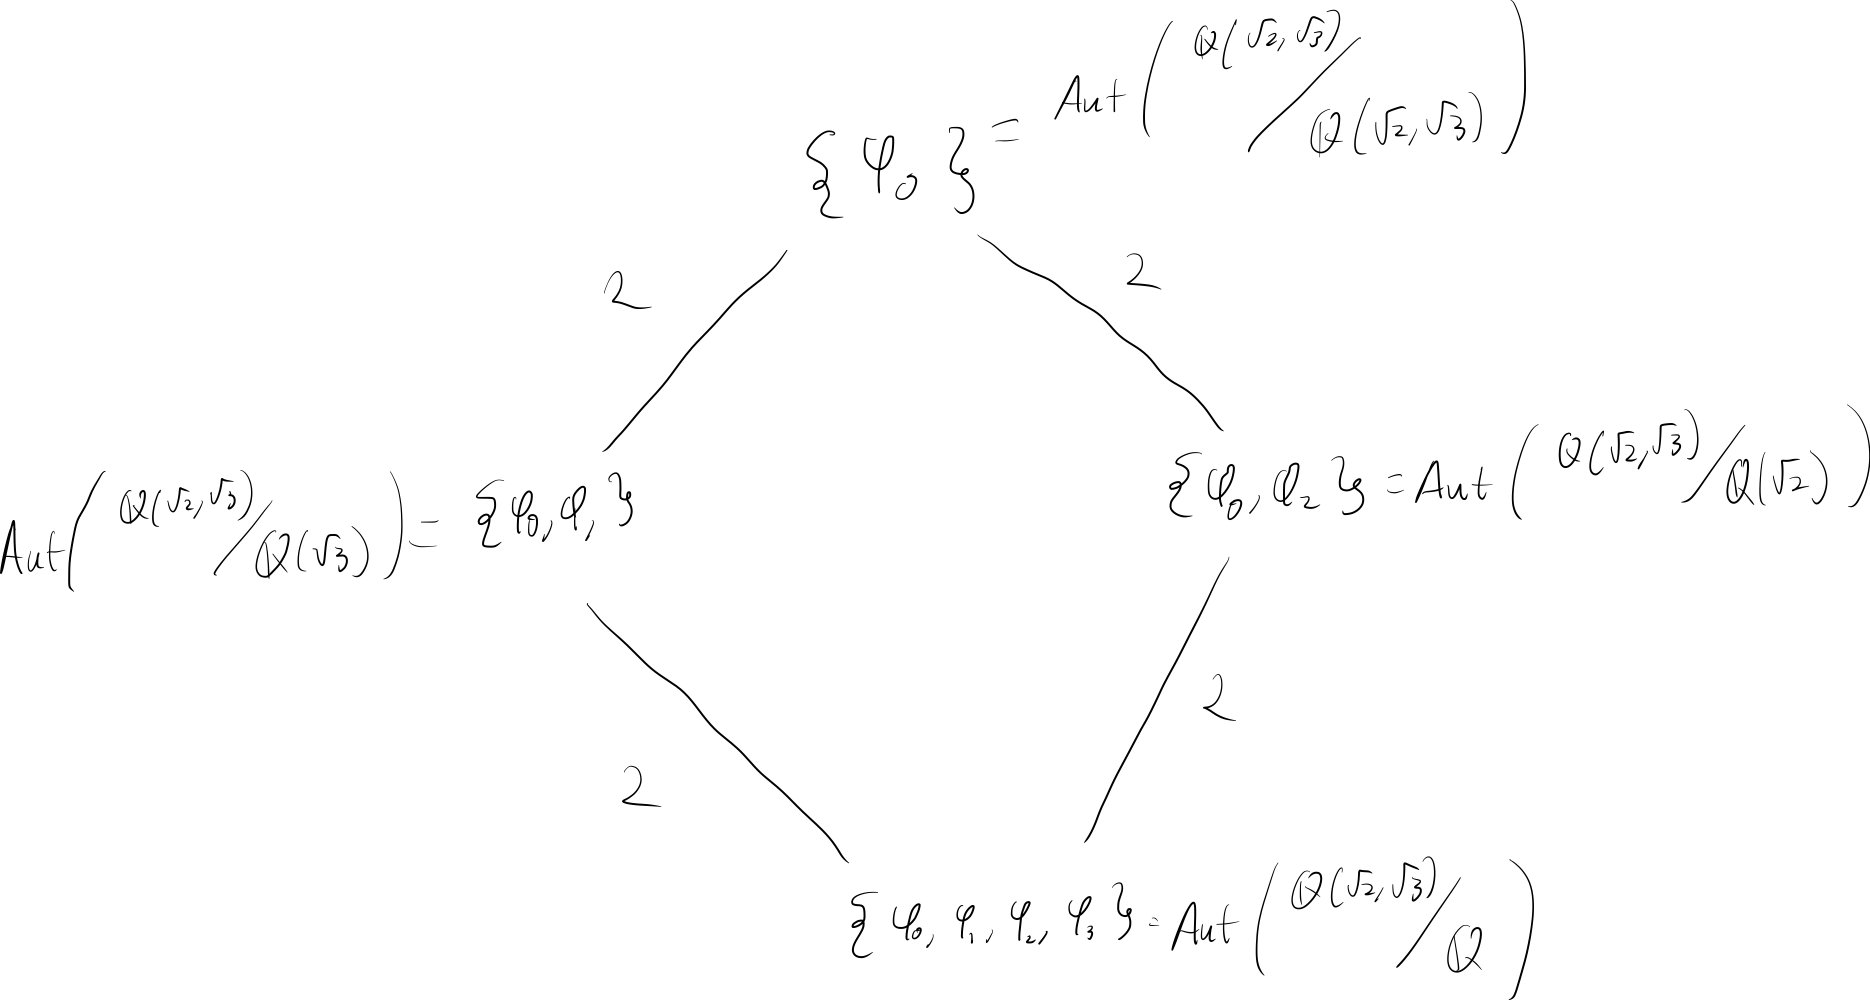
\includegraphics[width=\textwidth]{images/automorphism_lattice.png}
  %\end{center}
  % automorphism group lattice
  \subsection{Example: A Cubic Polynomial}%
  Consider the function $f(x) = x^3 - 2$. The function has one real root, $r_1=\sqrt[3]{2}$, and two complex roots. Let's examine $\Q(\sqrt[3]{2}) = \{a + b\sqrt[3]{2} + c\sqrt[3]{4}\mid a,b,c\in\Q\}$; $r_2$ and $r_3$ are not in $Q(\sqrt[3]{2})$. We could instead consider $\Q(\sqrt[3]{2},r_1,r_2)$.
  \begin{align*}
    x^3-2 &= (x-r_1)(x^2 + r_1x + r_1^2)\\
    r_2 &= \frac{-r_1 + \sqrt{r_1^2-4r_1^2}}{2}\\
        &= r_1\frac{-1+\sqrt{-3}}{2}\\
        &= r_1\zeta_3\\
    r_3 &= r_1\frac{-1 - \sqrt{-3}}{2}\\
        &= r_1\zeta_3^2
  \end{align*}
  However, including $r_2$ and $r_3$ is excessive --- all we need is $\Q(\sqrt[3]{2},\zeta_3)$. Therefore, the basis of this vector space is $\{1,r_1,r_1^2,\zeta_3,\zeta_3 r_1,\zeta_3 r_1^2\}$ (note that $\zeta_3^2 = -1-\zeta_3$). Therefore, $\text{dim}_{\Q}\Q(\sqrt[3]{2},\zeta_3)=6$, and $\Q(\sqrt[3]{2},\zeta_3) = K(f)$.Additionally, we have $\text{Aut}(\Q(\sqrt[3]{2})/\Q) = \{\varphi_0\}$, but $\dim_{\Q}\Q(\sqrt[3]{2}) = 3$. For the full field extension, we need to find $\varphi(\sqrt[3]{2})$ and $\varphi(\zeta_3)$.
  \begin{align*}
    \varphi(\sqrt[3]{2}) &\in \{r_1,\zeta_3 r_1,\zeta_3^2 r_1\}\\
    \varphi(\zeta) &\in \{\zeta_3,\zeta_3^2\}\\
    \varphi_0 &: r_1\mapsto r_1,\zeta_3\mapsto \zeta_3\\
    \varphi_1 &: r_1\mapsto \zeta_3r_1,\zeta_3\mapsto \zeta_3\\
    \varphi_2 &: r_1\mapsto r_1,\zeta_3\mapsto \zeta_3^2\\
    \varphi_3 &: r_1\mapsto \zeta_3^2r_1,\zeta_3\mapsto \zeta_3\\
    \varphi_4 &: r_1\mapsto \zeta_3r_1,\zeta_3\mapsto \zeta_3^2\\
    \varphi_5 &: r_1\mapsto \zeta_3^2r_1,\zeta_3\mapsto \zeta_3^2\\
    \shortintertext{Therefore,}
    \text{Aut}(\Q(\sqrt[3]{2},\zeta_3)/\Q) &= 6\\
                                           &= \dim_{\Q}\Q(\sqrt[3],\sqrt[3]{2})
  \end{align*}
  \section{Rings}%
  Consider the integers under the normal operations, $(\Z,+,\cdot)$; this will serve as the motivation for rings in the future.
  \subsection{Definition of a Ring}%
   Let $R$ be a nonempty set with operations $(+,\cdot)$, with the following properties:
    \begin{enumerate}[(1)]
      \item $(R,+)$ is an abelian group:
        \begin{itemize}
          \item Closed: $r_1 + r_2\in R,~ \forall r_1,r_2\in R$
          \item Identity: $\exists 0_R,~r + 0_R = 0_R+r = r$
          \item Associativity: $r_1 + (r_2 + r_3) = (r_1 + r_2) + r_3$
          \item Inverse: $\forall r\in R,~\exists -r\in R, r + (-r) = 0_R$
          \item Commutativity: $r_1 + r_2 = r_2 + r_1$
        \end{itemize}
      \item Closure under Multiplication: $r_1\cdot r_2\in R,~\forall r_1,r_2\in R$
      \item Associativity under Multiplication: $r_1\cdot (r_2 \cdot r_3) = (r_1\cdot r_2)\cdot r_3$
      \item Distributivity: $r_1\cdot (r_2 + r_3) = r_1\cdot r_2 + r_2\cdot r_3, (r_1 + r_2)\cdot r_3 = r_1\cdot r_3 + r_2\cdot r_3$
    \end{enumerate}
  We say $(R,+,\cdot)$ is a ring if it satisfies all these properties.\\

  If $\exists 1_R\in R$ such that $r\cdot 1_R = 1_R \cdot r = r$, then we say $R$ is a ring with identity, and $1_R$ is the multiplicative identity. If multiplication is commutative, then $R$ is known as a commutative ring.
  \subsubsection{Examples}%
  \begin{enumerate}[(1)]
    \item $(\Z,+,\cdot)$, $(\Q,+,\cdot)$, $(\R,+,\cdot)$, $(\mathbb{C},+,\cdot)$ are commutative rings with identity value of $1$.
    \item $(\Z/n\Z,+,\cdot)$ is a commutative ring with identity $1_{R} = [1]_n$.
    \item $(\R[x],+,\cdot)$, where $\displaystyle\R[x] = \left\{\sum_{i=0}^{n}a_ix^i\mid a_i\in\R\right\}$, is a commutative ring with identity.
    \item $(2\Z,+,\cdot)$ is a commutative ring \textit{without} identity.
    \item $(\text{Mat}_{n}(\R),+,\cdot)$, where $\text{Mat}_n(\R)$ refers to $n\times n$ matrices with real entries, is a \textit{non}commutative ring with identity.
  \end{enumerate}
  \subsection{Division Rings and Fields}%
  Let $R$ be a ring with identity. We say $R$ is a \textit{division ring} if $\forall r\in R\setminus \{0_R\}$, $\exists r^{-1}\in R$ with $r\cdot r^{-1} = 1_R = r^{-1}\cdot r$. If $R$ is also commutative, then $R$ is a \textit{field}.
  \subsubsection{Examples}%
  \begin{enumerate}[(1)]
    \item $(\Q,+,\cdot)$, $(\R,+,\cdot)$, and $(\mathbb{C},+,\cdot)$ are all fields.
    \item Let $p$ be prime, and set $F = \Z/p\Z$. Then, $F$ is a field; we denote this $\mathbb{F}_p$.
    \item Define 
      \begin{align*}
        \mathbb{H} = \{a+bi+cj+dk\mid a,b,c,d\in\R,i^2=j^2=k^2=-1,ij=k=-ji,jk=i=-kj,ki=j=-ik\}.
      \end{align*}
      Then, $\mathbb{H}$ is a division ring, known as the Hamiltonian quaternions. Note that $\mathbb{C}\subset \mathbb{H}$.
  \end{enumerate}
  \subsection{Properties of Rings}%
  \begin{description}
    \item[Proposition 4.1:] Let $R$ be a ring.
      \begin{enumerate}[(1)]
        \item $0_R a = a0_r = 0$ $\forall a\in R$
        \item $(-a)b = a(-b) = -(ab)$ $\forall a,b\in R$
        \item $(-a)(-b) = ab$ $\forall a,b\in R$
        \item If $\exists 1_R\in R$, then $1_R$ is unique, and $-a = (-1_R)a$.
      \end{enumerate}
    \item[Proof of (1):] Let $a\in R$. Then,
      \begin{align*}
        0_Ra &= (0_R + 0_R)a \tag*{Additive Inverse}\\
        0_Ra &= 0_Ra + 0_Ra \tag*{Distributivity}\\
        0_Ra + (-0_Ra) &= 0_Ra + 0_Ra (-0_Ra)\\
        0_R &= 0_Ra. \tag*{Additive Inverse}
      \end{align*}
    \item[Proof of (2):] Let $a,b\in R$. Note that $-(ab)$ is the unique inverse such that $ab + (-(ab)) = 0_R$ via group theory. We have
      \begin{align*}
        ab + (-a)b &= (a+(-a))b \tag*{Distributivity}\\
                   &= (0_R)b\tag*{Additive Inverse}\\
                   &= 0_R. \tag*{By Property (1)}
      \end{align*}
      Thus, $(-a)b = -(ab)$.
  \end{description}
  \subsection{Zero Divisor and Units in Rings}%
    Let $a\in R$, $a\neq 0_R$. If $\exists b\in R$ with $b\neq 0_R$ such that $ab = 0_R = ba$, then we say $a$ is a zero divisor.\\

    If $1_R \in R$, we say $u\in R$ is a unit if $\exists v\in R$ (can be equal to $u$) with $uv = 1_R = vu$. The collection of units in $R$ is denoted $R^{\times}$.
    \begin{description}
      \tiny
      \item[Exercise:] Show that $R^{\times}$ is a group under multiplication.
    \end{description}
    \subsubsection{Examples}%
  \begin{enumerate}[(1)]
    \item Let $R = \Z/6\Z$. Note that $[2]_6 [3]_{6} = [6]_{6} = [0]_{6}$, so both $[2]_6$ and $[3]_{6}$ are both zero divisors. Additionally, $[4]_6[3]_6 = [6]_{6} = [0]_{6}$. Meanwhile, since $(\Z/6\Z)^{\times}=\{[1]_{6},[5]_{6}\}$, those are the two units of $\Z/6\Z$.
    \item $\Z$ has no zero divisors. $\Z^{\times} = \{\pm 1\}$.
    \item $\Q$ has no zero divisors. $\Q^{\times} = \Q\setminus \{0\}$.
    \item $\Z[i] = \{a+bi\mid a,b\in\Z,i^2=-1\}$ has no zero divisors (as $\mathbb{C}$ is a field). $\Z[i]^{\times} = \{\pm 1,\pm i\}$.
  \end{enumerate}
  \subsection{Subrings}%
  Let $(R,+,\times)$. If $S\subseteq R$ is a nonempty subset, and $(S,+,\cdot)$ is a ring, then $S$ is a subring of $R$. To see $S$ is a subring, it is enough to show:
  \begin{itemize}
    \item $S\neq \emptyset$.
    \item $S$ is closed under subtraction.
    \item $S$ is closed under multiplication of elements in $S$.
  \end{itemize}
  \subsubsection{Examples}%
  \begin{enumerate}[(1)]
    \item 
    \begin{align*}
      \underbrace{\Z\subseteq\Q\subseteq\R\subseteq \C}_{\text{subrings}}
    \end{align*}
  \item $\R\subseteq \R[x]$ is a subring.
  \item $S = \{[0]_4,[2]_4\}\subseteq \Z/4\Z$ is a subring.
  \end{enumerate}
  \subsection{Integral Domains}%
  Let $R$ be a commutative ring with identity. We say $R$ is an integral domain if $R$ has no zero divisors.
  \subsubsection{Examples}%
  \begin{enumerate}[(1)]
    \item $\Z$, the integers, is an integral domain, that is not a field.
    \item All fields are integral domains.
    \item $\Z/6\Z$ is \textit{not} an integral domain, as it has zero divisors.
    \item $\Z/n\Z$ is not an integral domain if $n$ is composite.
  \end{enumerate}
  Integral domains are nice due to allowance of cancellations. For example, if $2m = 2n$ in $\Z$, then we find $2(m-n) = 0$, and since $\Z$ has no zero divisors, it must be the case that $m=n$.\\

  However, in a ring that is not an integral domain, such as $\Z/6\Z$, we cannot use the same technique to find the solution to a similar equation. For example, $3\cdot 2 = 0 = 3\cdot 4$, but $2\neq 4$.
  \subsubsection{Proposition: Equations in Integral Domains}%
  Let $R$ be an integral domain. If $a,b,c\in R$ with $a\neq 0_R$, and $ab = ac$, then $b=c$.\\

  \textbf{Proof:}
  \begin{align*}
    ab &= ac\\
    a(b-c) &= 0_R\\
    \shortintertext{Since $a\neq 0$,}
    b-c &= 0_R\\
    b &= c.
  \end{align*}
  \subsubsection{Theorem: Finite Integral Domains and Fields}%
  If $R$ is an integral domain, and $\card(R) < \infty$ ,then $R$ is a field.\\

  \textbf{Proof:} Let $a\in R$, $a\neq 0_{R}$. Note $ab \neq 0_R$ for all $b\in R,~b\neq 0_R$.\\

  Define $\varphi_a: R\setminus\{0_R\} \rightarrow R\setminus\{0_R\}$, $b\mapsto ab$. If $\varphi_a(b) = \varphi_a(c)$, then $ab = ac$, and by our previous result, $b=c$ --- therefore, $\varphi_a$ is injective.\\

  Since $R\setminus \{0_R\}$ is finite, and $\varphi_a$ is injective, then $\varphi_a$ is surjective. In particular, this means $\exists b\in R\setminus\{0_R\}$ with $\varphi_a(b) = 1_R$; therefore, $ab = 1_R$. Since $R$ is commutative, $ba = 1_R$, so $b = a^{-1}$.
  \subsubsection{Examples of Abstract Rings}%
  
  \subsubsection{Ring of Integers in a Field}%
  Let $d\in \Z$, $d$ is square-free (there is no square that divides $d$). Set $\Q(\sqrt{d}) = \{a + b\sqrt{d}\mid a,b\in\Q\} \subseteq \C$. This is a field (can be verified as a subfield of $\C$).\\

  We can define
  \begin{align*}
    \mathcal{O}_{\Q\left(\sqrt{d}\right)} &= \begin{cases}
      \Z[\sqrt{d}] = \{a + b\sqrt{d}\mid a,b\in\Z\} & d \equiv 2,3\mod 4\\
      \Z\left[\frac{1 + \sqrt{d}}{2}\right] = \{a + b\left(\frac{1+\sqrt{d}}{2}\right)\mid a,b\in\Z\} & d\equiv 1\mod 4
    \end{cases}.
  \end{align*}
  Then, $\mathcal{O}_{\Q(\sqrt{d})}$ is a subring of $\Q(\sqrt{d})$. This is known as the ring of integers of $\Q(\sqrt{d})$. This set behaves in $\Q(\sqrt{d})$ the same say that $\Z$ does inside $\Q$. The set $\mathcal{O}_{\Q(\sqrt{d})}$ is the collection of all roots in $\Q(\sqrt{d})$ of monic (coefficient of highest degree is 1) polynomials with coefficients in $\Z$.\\

  For example, if $d = -1$, defining $\Q(i)$, then we can verify that $\Z[i]$ is a root of a monic polynomial with coefficients in $\Z$.
  \subsubsection{Ring of Matrices}%
  Let $R$ be a ring. Then,
  \begin{align*}
    \text{Mat}_{n}(R) &= \{\text{$n\times n$ matrices with entries in $R$}\}
  \end{align*}
  is a ring under matrix addition and multiplication.
  \subsubsection{Ring of Functions}%
  Let $L^{1}(\R)$ be all functions $f: \R\rightarrow\R$ such that
  \begin{align*}
    \int_{\R}|f(x)|dx
  \end{align*}
  exists. The set $L^{1}(\R)$ is a ring under pointwise addition and convolution, where convolution is defined as
  \begin{align*}
    \left(f\ast g\right)(x) &= \int_{\R}f(x-y)g(y)dy.
  \end{align*}
  This is a commutative ring without identity.
  \subsubsection{Group Ring}%
  Let $K$ be a field and $G$ a group. Set $K[G]$ to be all formal linear combinations of the form
  \begin{align*}
    \alpha = \sum_{x\in G} a_x x,
  \end{align*}
  with $a_x\in K$, $x\in G$, with $a_x = 0$ for all but finitely many $x$.\\

  Given
  \begin{align*}
    \alpha &= \sum_{x\in G}a_x x\\
    \alpha &= \sum_{y\in G}b_y y,
  \end{align*}
  define
  \begin{align*}
    \alpha + \beta &= \sum_{x\in G}(a_x + b_x) x\\
    \alpha\beta &= \sum_{x\in G}\sum_{y\in G}a_xb_yxy\\
                &= \sum_{z\in G}\left(\sum_{xy=z}a_xb_y\right)z.
  \end{align*}
  This is a ring under these operations, known as the group ring. It is commutative if and only if $G$ is abelian.
  \subsubsection{Polynomials under a Ring}%
  Let $R$ be a ring. Set
  \begin{align*}
    R[x] = \left\{\sum_{i=1}^{n}a_ix^i\mid a_i\in R,n\in \Z_{\geq 0}\right\}
  \end{align*}
  to be the all polynomials with coefficients in $R$. This is a ring under polynomial addition and multiplication. If $R$ is commutative, then $R[x]$ is commutative.\\

  \subsubsection{Proposition: Polynomial Properties}%
  Let $R$ be an integral domain, with $p(x),q(x)\in R[x]\setminus\{0\}$. Then:
  \begin{enumerate}[(1)]
    \item $\text{deg}(p(x)q(x)) = \text{deg}(p(x)) + \text{deg}(q(x))$
    \item $R[x]^{\times} = R^{\times}$
    \item $R[x]$ is an integral domain.
  \end{enumerate}
  \begin{description}
    \item[Proof of (1):] Let
      \begin{align*}
        p(x) &= a_mx^m + \cdots + a_1x + a_0\\
        q(x) &= b_nx^n + \cdots + b_1x + b_0
      \end{align*}
      with $a_m,b_n\neq 0$ --- $\text{deg}(p) = m$ and $\text{deg}(q) = n$. Then,
      \begin{align*}
        p(x)q(x) = a_mb_nx^{m+n} + \text{lower degree terms},
      \end{align*}
      and since $a_mb_n\neq 0$ as $R$ is an integral domain with $a_m,b_n\neq 0$, $\text{deg}(pq) = m+n$.
  \end{description}
  \subsection{Ring Homomorphism}%
  Let $R$ and $S$ be rings. A ring homomorphism between $R$ and $S$ is a map $\varphi: R\rightarrow S$ that satisfies the following properties for all $r_1,r_2\in R$:
  \begin{enumerate}[(1)]
    \item $\displaystyle\varphi\left(r_1 +_{\tiny R} r_2\right) = \varphi(r_1) +_{\tiny S} \varphi(r_2)$
    \item $\displaystyle\varphi \left(r_1 \cdot_{\tiny R} r_2\right) = \varphi(r_1) \cdot_{\tiny S} \varphi(r_2)$
  \end{enumerate}
  The kernel of a ring homomorphism $\varphi$ is given by
  \begin{align*}
    \ker(\varphi): \{r\in R\mid \varphi(r) = 0_S\}
  \end{align*}
  A bijective ring homomorphism is called an isomorphism. If there exists such a bijection between $R$ and $S$, we say $R$ and $S$ are isomorphic.\\

  If $\varphi$ is an isomorphism, we write
  \begin{align*}
    \varphi: R\xrightarrow{\simeq}S
  \end{align*}
  \subsection{Examples: Ring Homomorphisms}%
  \subsubsection{Not a Ring Homomorphism}%
  Let $R = \Z$ and $S = 2\Z$. Define
  \begin{align*}
    \varphi: \Z&\rightarrow 2\Z\\
    n&\mapsto 2n.
  \end{align*}
  Let $m,n\in\Z$. We have
  \begin{align*}
    \varphi(m+n) &= 2(m+n)\\
                 &= 2m + 2n\\
                 &= \varphi(m) + \varphi(n).
  \end{align*}
  However,
  \begin{align*}
    \varphi(mn) &= 2(mn)\\
    \varphi(m)\varphi(n) &= 4(mn).
  \end{align*}
  \subsubsection{Homomorphism between Integers and Integers Modulo $n$}%
  Consider $R = \Z$ and $S = \Z/n\Z$. Define
  \begin{align*}
    \varphi:\Z&\rightarrow \Z/n\Z\\
    a&\mapsto [a]_{n}.
  \end{align*}
  Let $a,b\in\Z$. We have
  \begin{align*}
    \varphi(a+b) &= [a+b]_{n}\\
                 &= [a]_{n} + [b]_n\\
                 &= \varphi(a) + \varphi(b).
  \end{align*}
  Additionally, we have
  \begin{align*}
    \varphi(ab) &= [ab]_n\\
                &= [a]_n[b]_n\\
                &= \varphi(a)\varphi(b).
  \end{align*}
  So, $\varphi$ is a ring homomorphism. Note that
  \begin{align*}
    \ker(\varphi) &= \{a\in \Z\mid \varphi(a) = [0]_n\}\\
                  &= \{a\in \Z\mid [a]_n = [0]_n\}\\
                  &= \{a\in \Z\mid n | a\}\\
                  &= n\Z.
  \end{align*}
  \subsubsection{Homomorphism Between the Polynomials and Reals}%
  Let $S = \R[x]$ and $T = \R$. Define
  \begin{align*}
    \varphi_{a}: \R[x]&\rightarrow \R\\
    f&\mapsto f(a)\\
  \end{align*}
  Let $f(x),g(x) = \R[x]$. Then,
  \begin{align*}
    \varphi_a(f(x) + \varphi(g)(x)) &= \varphi_a((a_0 + b_0) + \cdots + (a_m + b_m)x^m + b_{m+1}x^{m+1} + \cdots b_nx^n)\\
                                    &= (a_0 + b_0) + \cdots + (a_m + b_m)a^m + b_{m+1}a^{m+1} + \cdots + b_na^n\\
                                    &= \varphi_a(f(x)) + \varphi_a(g(x)).
  \end{align*}
  Similarly, we can verify that $\varphi_a(f(x)g(x)) = \varphi_a(f(x))\varphi_a(g(x))$. So, $\varphi_a$ is a ring homomorphism. Note that
  \begin{align*}
    \ker(\varphi_a) &= \{f(x)\in \R[x]\mid f(a) = 0\}\\
                    &= \{f(x)\in \R[x]\mid (x-a)|f(x)\}\\
                    &= (x-a)\R[x]
  \end{align*}
  \subsubsection{Homomorphism between Matrices}%
  Define
  \begin{align*}
    R &= \left\{ \begin{bmatrix}a&b\\0&d\end{bmatrix}\in \text{Mat}_{2}(\R)\right\}\\
    S &= \R,
  \end{align*}
  and
  \begin{align*}
    \varphi:R&\rightarrow S\\
    \begin{bmatrix}a&b\\0&d\end{bmatrix}&\mapsto a.
  \end{align*}
  Then,
  \begin{align*}
    \varphi \left(\begin{bmatrix}a_1&b_1\\0&d_1\end{bmatrix}+\begin{bmatrix}a_2&b_2\\0&d_2\end{bmatrix}\right) &= \varphi \left(\begin{bmatrix}a_1+a_2&b_1+b_2\\0&d_1+d_2\end{bmatrix}\right)\\
                                    &= a_1 + a_2\\
                                    &= \varphi \left(\begin{bmatrix}a_1&b_1\\0&d_1\end{bmatrix}\right) + \varphi \left(\begin{bmatrix}a_2&b_2\\0&d_2\end{bmatrix}\right),
  \end{align*}
  and
  \begin{align*}
    \varphi \left(\begin{bmatrix}a_1&b_1\\0&d_1\end{bmatrix}\begin{bmatrix}a_2&b_2\\0&d_2\end{bmatrix}\right) &= \varphi \left(\begin{bmatrix}a_1a_2&a_1b_2 + b_1d_2\\0&d_1d_2\end{bmatrix}\right)\\
                                    &= a_1 a_2\\
                                    &= \varphi \left(\begin{bmatrix}a_1&b_1\\0&d_1\end{bmatrix}\right)  \varphi \left(\begin{bmatrix}a_2&b_2\\0&d_2\end{bmatrix}\right).
  \end{align*}
  So $\varphi$ is a ring homomorphism that is surjective but not injective. Note
  \begin{align*}
    \ker(\varphi) &= \left\{ \begin{bmatrix}0&b\\0&d\end{bmatrix}\mid b,d\in\R\right\}.
  \end{align*}
  \subsubsection{Proposition: Fundamental Theorem of Ring Homomorphisms}%
  Let $\varphi: R\rightarrow S$ be a ring homomorphism.
  \begin{enumerate}[(1)]
    \item The image of $\varphi$, $\varphi(R) = \{s\in S\mid s = \varphi(r)\text{ for some }r\in R\}$, is a subring of $S$.
    \item The kernel, $\ker(\varphi)$, is a subring of $R$.\\

      Additionally, for any $r\in R$, and $a\in \ker(\varphi)$, $ar\in \ker(\varphi)$ and $ra\in \ker(\varphi)$.
  \end{enumerate}
  \begin{description}
    \item[Proof of (2):] To show $\ker(\varphi)$ is a subring, we must show that $\ker(\varphi)$ is non-empty, closed under subtraction, and closed under multiplication.\\

      First, since $\varphi(0_R) = 0_S$ (verify this), $\ker(\varphi)$ is non-empty.\\

      Let $a,b\in\ker(\varphi)$. We have
      \begin{align*}
        \varphi(a-b) &= \varphi(a + (-b))\\
                     &= \varphi(a) + \varphi(-b)\\
                     &= \varphi(a)-\varphi(b) \tag*{check $\varphi(-b) = -\varphi(b)$}\\
                     &= 0_S - 0_S\\
                     &= 0_S.
      \end{align*}
      Thus, $a-b\in\ker(\varphi)$, and $\ker(\varphi)$ is closed under subtraction.\\

      To show $\ker(\varphi)$ is closed under multiplication, we will prove the general case. Let $a\in\ker(\varphi)$ and $r\in R$. We have
      \begin{align*}
        \varphi(ra) &= \varphi(r)\varphi(a)\\
                    &= \varphi(r)0_S\\
                    &= 0_S.
      \end{align*}
      Similarly, $\varphi(ar) = 0_S$. So, $ar,ra\in\ker(\varphi)$.
  \end{description}
  The stronger condition that we found for $\ker(\varphi)$ (closed under multiplication of all elements of the ring, not merely those from the subring) forms what we call an ideal.
  \subsection{Quotient Rings}%
  \subsubsection{Defining an Equivalence Relation on a Ring}%
  Set $K = \ker(\varphi)$. We will define a relation on $R$, $\sim$, where $r_1 \sim r_2$ if $r_1-r_2\in K$. We want to see if $\sim$ is an equivalence relation:
  \begin{itemize}
    \item Reflexive: $r\sim r$ since $r-r=0_R \in K$.
    \item Symmetric: $r_1\sim r_2$ implies $r_1 - r_2 = k$ for some $k\in K$. Since $k$ is a subring, $-k\in K$, so $r_2 - r_1\in K$.
    \item Transitive: suppose $r_1 \sim r_2$ and $r_2\sim r_3$. This means there are elements $k_1,k_2\in K$ with $r_1-r_2 = k_1$ and $r_2-r_3 = k_2$. Since $K$ is a subring, $(r_1 - r_2) + (r_2 - r_3) = r_1 - r_3 = k_1 + k_2\in K$. Thus, $r_1 \sim r_3$.
  \end{itemize}
  Since $\sim$ is reflexive, symmetric, and transitive, $\sim$ is an equivalence relation on $R$.\\
  
  Since $\sim$ is an equivalence relation on $R$, we will want to examine equivalence classes of $R$ under $\sim$. Specifically, for $r\in R$, we have
  \begin{align*}
    [r]_K &= \{\tilde{r}\in R \mid r-\tilde{r}\in K\}\\
          &= \{\tilde{r}\in R \mid r - \tilde{r} = k\text{ for some }k\in K\}\\
          &= \{r + k\mid k\in K\}\\
          &= r+K.
  \end{align*}
  We will define the set
  \begin{align*}
    R/K = \{r + K\mid r\in R\}
  \end{align*}
  to be the set of all equivalence classes.
  \begin{description}
    \item[Example:] Let $\varphi: \Z\rightarrow \Z/n\Z$, $a\mapsto [a]_n$. Then, $\ker(\varphi) = n\Z$. Then, $R/K = \Z/n\Z$.
  \end{description}
  Let $r_1 + K,r_2+K\in R/K$. The new question is whether or not we can define addition and multiplication on $R/K$. Suppose that the following are the definition of multiplication and addition on $R/K$.
  \begin{align*}
    (r_1 + K) + (r_2 + K) &= (r_1 + r_2) + K\\
    (r_1 + K)(r_2 + K) &= (r_1r_2) + K.
  \end{align*}
  Suppose $r_1 + K = \tilde{r_1} + K$ and $r_2 + K = \tilde{r_2} + K$. This means there are $k_1,k_2\in K$ with $r_1 - \tilde{r_1} = k_1$, $r_2 - \tilde{r_2} = k_2$, or that $r_1 = \tilde{r_1} + k_1$, $r_2 = \tilde{r_2} + k_2$.\\

  To see if the map is well-defined, we have
  \begin{align*}
    (r_1 + K) + (r_2 + K) &= (r_1 + r_2) + K\\
                          &= (\tilde{r_1} + k_1 + \tilde{r_2} + k_2) + K\\
                          &= (\tilde{r_1} + k_1) + K + (\tilde{r_2} + k_2) + K\\
                          &= (\tilde{r_1} + K) + (\tilde{r_2} + K)\\
    \shortintertext{since $\tilde{r_1} + k_1 - \tilde{r_1} = k\in K$.}
  \end{align*}
  Thus, our addition is well-defined.\\

  Examining multiplication, we see that
  \begin{align*}
    (r_1 + K)  (r_2 + K) &= r_1r_2 + K\\
                         &= (\tilde{r_1} + k_1)(\tilde{r_2} + k_2) + K\\
                         &= \tilde{r_1}\tilde{r_2} + \underbrace{k_1\tilde{r_2} + \tilde{r_1}k_2 + k_1k_2}_{\in K \text{ since $K = \ker(\varphi)$}} + K\\
                         &= \tilde{r_1}\tilde{r_2} + K.
  \end{align*}
  Therefore, our multiplication is well-defined.\\

  We can show that $R/K$ is a ring (verify for yourself).
  \begin{description}
    \small
    \item[Note:] This construction would not have worked if $K$ was merely a subring, as multiplication would not be well-defined.
  \end{description}
  \subsubsection{Ideals}%
  Let $I\subseteq R$ be a subring.
  \begin{enumerate}[(1)]
    \item If $ra\in I$ for every $r \in R$, we say $I$ is a left-ideal of $R$.
    \item If $ar\in I$ for every $r\in R$, then we say $I$ is a right-ideal of $R$.
    \item If $I$ is a left-ideal and a right-ideal of $R$, then we say $I$ is an ideal of $R$.
  \end{enumerate}
  If $I\subseteq R$ is an ideal, we define $r_1\sim_{I}r_2$ if $r_1-r_2 \in I$, and $R/I = \{r+I\mid r\in I\}$. Addition and multiplication in $R/I$ are defined as
  \begin{align*}
    (r_1 + I) + (r_2 + I) &= (r_1 + r_2) + I\\
    (r_1 + I)(r_2 + I) &= r_1r_2 + I.
  \end{align*}
  \subsubsection{Examples of Ideals}%
  \begin{enumerate}[(1)]
    \item $n\Z\subseteq \Z$ is an ideal; if $nk\in n\Z$, and $m\in\Z$, then $m(nk) = n(mk) \in n\Z$.
    \item Let $R = \Z[x]$. Set $\langle x^2\rangle = \{f(x)x^2\mid f(x)\in \Z[x]\}$. This is an ideal.
    \item Let $R$ be a ring. If $r\in R$, we define $\langle r \rangle = \{ar \mid a\in R\}$.
    \item Set $I = \{(2n,0)\mid n\in\Z\}$ in $\Z\times\Z$. Let $(a,b)\in \Z\times\Z$. Then, $(a,b)(2n,0) = (2an,0)\in I$, meaning $I$ is an ideal.
    \item Define $R = \left\{ \begin{bmatrix}a&b\\0&d\end{bmatrix}\in \text{Mat}_{2}(\R)\right\}$. Consider $I = \left\{ \begin{bmatrix}a&0\\0&d\end{bmatrix}\mid a,b\in\R\right\}$. Then,
      \begin{align*}
        \begin{bmatrix}a&b\\0&d\end{bmatrix} \begin{bmatrix}s&0\\0&t\end{bmatrix} &= \begin{bmatrix}as & bt\\0&dt\end{bmatrix}\\
        \begin{bmatrix}s&0\\0&t\end{bmatrix}\begin{bmatrix}a&b\\0&d\end{bmatrix} &= \begin{bmatrix}sa & sb\\0&td\end{bmatrix}.
      \end{align*}
      Therefore, $I$ is a subring but not an ideal.
    \item Let $R = \Z[x]$. Consider $I = \langle 2,x\rangle = \{2f(x) + g(x)\mid f(x),g(x)\in \Z[x]\}$. Then,
      \begin{align*}
        (2f_1(x) + xg(x))(2f_2(x) + xg_2(x)) &= 2\left(f_1(x)(2f_2(x) + xg_2(x))\right) + x(g_1(x)(2f_2(x) + xg_2(x)))\\
        h(x)\left(2f(x) + xg(x)\right) &= 2(f(x)h(x)) + x(g(x)h(x)),
      \end{align*}
      meaning $I$ is an ideal.
  \end{enumerate}
  \subsubsection{Examples of Quotient Rings}%
  \begin{enumerate}[(1)]
    \item Let $R = \Z$, $I = n\Z$. Then, $R/I = \Z/n\Z$.
    \item Let $R = \R[x]$, $I = \langle x^2\rangle$ as defined earlier. Then,
      \begin{align*}
        R/I &= \R[x]/\langle x^2\rangle\\
            &= f(x) + \langle x^2 \rangle.\\
            \shortintertext{Other examples include}
        f(x) &= a_nx^n + \cdots + a_1x + a_0 \in \R[x]\\
        f(x) + \langle x^2 \rangle &= a_1 x + a_0 + \langle x^2 \rangle \in \R[x]/\langle x^2\rangle\\
        \R[x]/\langle x^2\rangle &= \{a+bx + \langle x^2 \rangle\mid a,b\in\R\}.\\
        (a+bx + \langle x^2 \rangle)(c + dx \langle x^2 \rangle) &= ac + ad x + bc x + bdx^2 + \langle x^2 \rangle\\
                                                                 &= (ac) + (ad + bc) x + \langle x^2 \rangle\\
        (x+\langle x^2\rangle)^2 &= x^2 + \langle x^2 \rangle\\
                                 &= \langle x^2 \rangle.
      \end{align*}
    \item Let $R = \Z\times\Z$, $I = \{(2n,0)\mid n\in\Z\}$. Then,
      \begin{align*}
        R/I &= \{(a,b) + I\mid a,b\in\Z\}.\\
        (a,b) + I &= ([a]_2,b) + I \tag*{where $[a]_2$ is $a$ modulo 2.}
      \end{align*}
      We would expect that $\varphi: \Z/2\Z\times \Z \rightarrow R/I$, $([a]_2,b)\rightarrow (a,b) + I$ is an isomorphism (verify for yourself).
  \end{enumerate}
  \subsubsection{Isomorphisms to Quotient Rings}%
  Let $R = \Z[x]$, $I = \langle 2,x\rangle$, $J = \langle 2 \rangle = \{2f(x)\mid f(x)\in\Z[x]\}$.
  \begin{align*}
    R/J &= \{f(x) + \langle 2 \rangle \mid f(x)\in \Z[x]\}\\
    f(x) + \langle 2 \rangle &= g(x) + \langle 2 \rangle\\
    \shortintertext{if $2|(f(x)-g(x))$, meaning all coefficients of $f(x)-g(x)$ are divisible by $2$. Therefore,}
    f(x) + \langle 2 \rangle &= 5 + 4x + 7x^2 - 5x^3 \langle 2 \rangle\\
                             &= (1 + (2)(2)) + 2(2x) + x^2 + 2(3x^2) -x^3 - 2(2x^3) + \langle 2 \rangle\\
                             &= 1 + x^2 - x^3 + \langle 2 \rangle\\
                             &= 1 + x^2 - 2(x^3) + x^3 + \langle 2 \rangle\\
                             &= 1 + x^2 + x^3 + \langle 2 \rangle.\\
    (1 + x + x^2 + \langle 2 \rangle) + (x + \langle 2 \rangle) &= 1 + 2x + x^2 + \langle 2 \rangle\\
                                                                &= 1 + x^2 + \langle 2 \rangle.\\
                                                                \shortintertext{Therefore, we can consider}
    \Z[x]/\langle 2 \rangle &= \Z[x]/2\Z[x]\\
                            &\cong \Z/2\Z.
  \end{align*}
  \begin{align*}
    R/I &= \Z[x]/\langle 2,x\rangle\\
    f(x) + \langle 2,x\rangle &= a_nx^n + \cdots + a_1 x + a_0 + \langle 2,x\rangle\\
                              &= a_0 + \langle 2,x \rangle\\
                              &= \begin{cases}
                                0 & 2|a_0\\
                                1 & 2\not| a_0
                              \end{cases},
                              \shortintertext{So, we can consider}
    \Z[x]/\langle 2,x\rangle &\cong \Z/2\Z.
  \end{align*}
  \subsubsection{Isomorphism Example: Complex Numbers to Matrices}%
  Consider the set
  \begin{align*}
    R = \left\{ \begin{bmatrix}a&b\\-b & a\end{bmatrix}\in \text{Mat}_{2}(\R)\right\}.
  \end{align*}
  We can verify that $R$ is a ring.\\

  Define
  \begin{align*}
    \varphi&: \C\rightarrow R\\
    a + bi &\mapsto \begin{bmatrix}a&b\\-b&a\end{bmatrix}.
  \end{align*}
  We can verify that $\varphi$ is a bijective map.\\

  Let $a+bi,c+di\in \C$. Then,
  \begin{align*}
    \varphi((a+bi) + (c+di)) &= \varphi((a+c) + (b+d)i)\\
                             &= \begin{bmatrix}a+c & b+ d\\-(b+d) & a+c\end{bmatrix}\\
                             &= \begin{bmatrix}a&b\\-b&a\end{bmatrix} + \begin{bmatrix}c & d\\-d&c\end{bmatrix}\\
                             &= \varphi(a+bi) + \varphi(c+di),\\
                             \shortintertext{and}
    \varphi((a+bi)(c+di)) &= \varphi((ac-bd) + (ad + bc)i)\\
                          &= \begin{bmatrix}ac-bd & ad + bc\\ -(ad + bc) & ac - bd\end{bmatrix}\\
    \varphi(a+bi)\varphi(c+di) &= \begin{bmatrix}a&b\\-b&a\end{bmatrix} \begin{bmatrix}c&d\\-d&c\end{bmatrix}\\
                               &= \begin{bmatrix}ac-bd & ad + bc\\-(ad+bc) & ac-bd\end{bmatrix}.
  \end{align*}
  Therefore, $\C\cong R$.
  \section{First Isomorphism Theorem}%
  Let $\varphi: R\rightarrow S$ be a homomorphism. We have $R/\ker\varphi \cong \varphi(R)$.
  \subsection{Proof of the First Isomorphism Theorem}%
  We want to show that $R/\ker(\varphi)\cong \varphi(R)$. Without loss of generality, assume $\varphi$ is surjective. Let $K = \ker(\varphi)$.\\

  We define $\Phi: R/K \rightarrow S$, $r+K\mapsto \varphi(r)$. We must show that $\Phi$ is a well-defined map. Let $r_1 + K = r_2 + K$ (meaning $r_1 - r_2 \in K$). This means $r_1 = r_2 + k$ for some $k\in K$. Applying $\Phi$, we have
  \begin{align*}
    \Phi(r_1 + K) &= \varphi(r_1)\\
                  &= \varphi(r_2 + k)\\
                  &= \varphi(r_2) + \varphi(k)\\
                  &= \varphi(r_2)\\
                  &= \Phi(r_2 + K).
  \end{align*}
  Let $r_1 + K$, $r_2 + K \in R/K$. Observe
  \begin{align*}
    \Phi((r_1 + K) + (r_2 + K)) &= \Phi((r_1 + r_2) + K)\\
                                &= \varphi(r_1 + r_2)\\
                                &= \varphi(r_1) + \varphi(r_2)\\
                                &= \Phi(r_1 + K) + \Phi(r_2 + K),
                                \intertext{and}
    \Phi((r_1 + K)(r_2 + K)) &= \Phi(r_1r_2 + K)\\
                             &= \varphi(r_1r_2)\\
                             &= \varphi(r_1)\varphi(r_2)\\
                             &= \Phi(r_1 + K)\Phi(r_2 + K),
  \end{align*}
  meaning $\Phi$ is a homomorphism.\\

  Let $s\in S$. Since $\varphi$ is surjective, there exists $r\in R$ with $\varphi(r) = s$. So, $\Phi(r+K) = \varphi(r) = s$. Thus, $\Phi$ is surjective.\\

  Let $r+K\in \ker(\Phi)$. Then,
  \begin{align*}
    \Phi(r+k) &= 0_S\\
              &= \varphi(r),
  \end{align*}
  meaning $r\in \ker(\varphi) = K$. So, $r+K = 0_{R} + K = 0_{R/K}$. Thus, $\Phi$ is injective.
  \subsection{Using the First Isomorphism Theorem: Example 1}%
  Let $\varphi: \Z[x]\rightarrow \Z/2\Z$, $a_0 + a_1x + \cdots + a_nx^n \mapsto [a_0]_2$.\\

  To apply the first isomorphism theorem, we must check that this is a ring homomorphism. Let
  \begin{align*}
    f &= a_0 + a_1 x + \cdots + a_mx^m\\
    g &= b_0 + b_1 x + \cdots + b_mx^m
  \end{align*}
  be elements in $\Z[x]$. Note that 
  \begin{align*}
    \varphi(f+g) &= \varphi((a_0 + b_0) + \cdots)\\
                 &= [a_0 + b_0]_2\\
                 &= [a_0]_2 + [b_0]_2\\
                 &= \varphi(f) + \varphi(g)
                 \intertext{and}
    \varphi(fg) &= \varphi((a_0b_0) + \cdots)\\
                &=[a_0b_0]_2\\
                &= [a_0]_2 + [b_0]_2\\
                &= \varphi(f)\varphi(g).
  \end{align*}
  So $\varphi$ is a homomorphism. Note that $\varphi(0) = [0]_2$ and $\varphi(1) = [1]_2$. The first isomorphism theorem gives that $\Z[x]/\ker\varphi \cong \Z/2\Z$.\\

  We claim that $\ker\varphi = \langle 2,x\rangle$.\\

  If $2f(x) + xg(x)\in \langle 2,x\rangle$, and we write $f(x) = a_0 + a_1 x + \cdots + a_nx^n$, then
  \begin{align*}
    \varphi(2f(x) + g(x)) &= \varphi(2)\varphi(f(x)) + \varphi(x)\varphi(g(x))\\
                          &= [0]_{2}[a_0]_2 + [0]_2\varphi(g(x))\\
                          &= [0]_2,
  \end{align*}
  so $\langle 2,x \rangle \subseteq \ker\varphi$.\\

  Let $f(x) = a_0 + a_1 x + \cdots + a_nx^n\in \ker(\varphi)$, meaning
  \begin{align*}
  [0]_2 &= \varphi(f(x))\\
        &= [a_0]_2.
  \end{align*}
  Therefore, $a_0 = 2k$. So,
  \begin{align*}
    f(x) &= 2k x(a_1 + a_2x + \cdots + a_nx^{n-1})\\
         &\in \langle 2,x\rangle.
  \end{align*}
  Thus, $\ker(\varphi)\subseteq \langle 2,x\rangle$, meaning $\ker(\varphi) = \langle 2,x\rangle$.\\

  By the first isomorphism theorem, $\Z[x]/\langle 2,x\rangle \cong \Z/2\Z$.
  \subsection{Using the First Isomorphism Theorem: Example 2}%
  We want to find the ring that is isomorphic to $(\Z\times\Z)/(2\Z\times 5\Z)$. We define
  \begin{align*}
    \varphi: \Z\times\Z \rightarrow \Z/2\Z \times \Z/5\Z\\
    (m,n)\mapsto ([m]_2,[n]_5).
  \end{align*}
  We will start by showing homomorphism as follows:
  \begin{align*}
    \varphi((m_1,n_1) + (m_2,n_2)) &= \varphi((m_1 + m_2,n_1+n_2))\\
                                   &= ([m_1 + m_2]_2,[n_1 + n_2]_5)\\
                                   &= ([m_1]_2 + [m_2]_2,[n_1]_5 + [n_2]_5)\\
                                   &= ([m_1]_2,[n_1]_5) + ([m_2]_2,[n_2]_5)\\
                                   &= \varphi((m_1,n_1)) + \varphi((m_2,n_2)),
     \intertext{and similarly for multiplication}
      \varphi((m_1,n_1)(m_2,n_2)) &= \varphi((m_1m_2,n_1n_2))\\
                                &= ([m_1m_2]_2,[n_1n_2]_5)\\
                                &\vdots\\
                                &= \varphi((m_1,n_1))\varphi((m_2,n_2))
  \end{align*}
  Let $([a]_2,[b]_5) \in \Z/2\Z\times\Z/5\Z$. Then, $\varphi((a,b)) = ([a]_2,[b]_5)$. Thus, $\varphi$ is surjective.\\

  Finally, we have $(m,n)\in \ker(\varphi)$ if and only if $[m]_2 = [0]_2$ and $[n]_5 = [0]_5$, meaning $m\in 2\Z$ and $n\in 5\Z$. Therefore, $\ker(\varphi) = 2\Z\times 5\Z$.
  \subsection{Using the First Isomorphism Theorem: Example 3}%
  Consider the map $\Z\rightarrow \Z/2\Z\times \Z/5\Z$, $n\mapsto ([n]_2,[n]_5)$. Note
  \begin{align*}
    \varphi(m+n) &= ([m+n]_2,[m+n]_5)\\
                 &= ([m]_2 + [n]_2,[m]_5 + [n]_5)\\
                 &= ([m]_2,[m]_5) + ([n]_2,[n]_5)\\
                 &= \varphi(m) + \varphi(n),
                 \intertext{and}
    \varphi(mn) &= \varphi(m)\varphi(n).
  \end{align*}
  We want to find if this map is surjective. Let $([a]_2,[b]_5)\in \Z/2\Z\times \Z/5\Z$. We are trying to find $n\in\Z$ such that $[n]_2 = [a]_2$ and $[n]_5 = [b]_5$, or $n\equiv a$ modulo 2 and $n\equiv b$ modulo 5.
  \begin{align*}
    n-a &\equiv 2k \text{ for some $k\in \Z$}\\
    n &\equiv a + 2k\\
    a+2k &\equiv b \text{ modulo 5}\\
    2k &= b-a \text{ modulo 5}\\
    k &= 3(b-a) \text{ modulo 5}\\
    n &= a + 2(3(b-a))\\
      &= a + 6(b-a).
  \end{align*}
  So $\varphi(a + 6(b-a)) = ([a]_2,[b]_5)$. Thus, $\varphi$ is surjective.\\

  Finally, we desire $\ker(\varphi)$. Observe that 
  \begin{align*}
    \ker(\varphi) &= \{n\in\Z \mid [n]_2=[0]_2,[n]_5=[0]_5\}\\
                  &= \{n\in\Z\mid 2|n,5|n\}\\
                  &= \{n\in\Z\mid 10|n\}\\
                  &= 10\Z.
  \end{align*}
  Thus, the first isomorphism theorem gives $\Z/10\Z \equiv \Z/2\Z \times \Z/5\Z$.
  \subsection{Proposition: Ring Homomorphisms and Ideals}%
  Let $R$ be a ring and $I\subseteq R$ be an ideal. The map
  \begin{align*}
    \varphi: R\rightarrow R/I\\
    r\mapsto r+I
  \end{align*}
  is a surjective ring homomorphism with $\ker(\varphi) = I$. The proof is left as an exercise to the reader.
  \subsection{Using the First Isomorphism Theorem: Example 3}%
  Let $A$ be a ring and $X$ be any non-empty set. Let $R$ be the set of functions from $X$ to $A$.\\

  We have $R$ is a ring.
  \begin{align*}
    (f+g)(x) &= f(x) +_{A} g(x)\\
    (fg)(x) &= f(x)\cdot_{A}g(x).
  \end{align*}
  Fix $x_0 \in X$. We define $E_{x_0}: R\rightarrow A$ by
  \begin{align*}
    E_{x_0}(f) &= f(x_0).
  \end{align*}
  We have
  \begin{align*}
    E_{x_0}(f+g) &= (f+g)(x_0)\\
                 &= f(x_0) + g(x_0)\\
                 &= E_{x_0}(f) + E_{x_0}(g)\\
                 \intertext{and}
    E(x_0)(fg) &= (fg)(x_0)\\
               &= f(x_0)g(x_0)\\
               &= E_{x_0}(f)E_{x_0}(g).
  \end{align*}
  Therefore, $E_{x_0}$ is a homomorphism. Additionally, $E_{x_0}$ is surjective, since we can find $f_a: X\rightarrow A$, $x\mapsto a$, meaning $E_{x_0}(f_a) = f_a(x_0) = a$.\\

  If $f\in \ker(E_{x_0})$, then $E_{x_0}(f) = 0_A$. However, $E_{x_0}(f) = f(x_0)$. Then,
  \begin{align*}
    \ker(\varphi) &= \{f: X\rightarrow A \mid f(x_0) = 0_A\}\\
                  &= \mathcal{M}_{x_0}.
  \end{align*}
  By the first isomorphism theorem, we can see that $R/\mathcal{M}_{x_0} \cong A$.
  \subsection{Other Isomorphism Theorems}%
  Let $R$ be a ring.
  \begin{description}
    \item[Diamond Isomorphism Theorem:] Let $A$ be a subring of $R$ and $I$ an ideal of $R$. Define $A + I = \{a+i\mid a\in A,i\in I\}$. This is an ideal of $R$. We also have that $A\cap I$ is an ideal in $A$, and $(A+I)/I \equiv A/A\cap I$.
  \end{description}
  % https://tikzcd.yichuanshen.de/#N4Igdg9gJgpgziAXAbVABwnAlgFyxMJZARgBoAmAXVJADcBDAGwFcYkQBBAHS4GN60AAgCSIAL6l0mXPkIoADKWLU6TVu1ESp2PASLklKhizaJO4ySAw7ZRMvKNrTnANSaVMKAHN4RUADMAJwgAWyRFEBwIJGItECDQ8JoopANVE3YeXgIvCwDgsMQySOjEAGYaY3UzLJy8+ILU5NKysUoxIA
  \begin{center}
    \begin{tikzcd}
                          & A+I                                    &              \\
    I \arrow[ru, "\simeq"] &                                        & A \arrow[lu] \\
                          & A\cap I \arrow[lu] \arrow[ru, "\simeq"] &             
    \end{tikzcd}
  \end{center}
  \begin{description}
    \item[Third Isomorphism Theorem:] Let $I,J$ be ideals of $R$ with $I\subseteq J$. Then, $J/I$ is an ideal of $R/I$ with $(R/I)/(J/I)\cong R/J$.
    \item[Lattice Isomorphism Theorem:] Let $I\subseteq R$ be an ideal. The correspondence $A\leftrightarrow A/I$ is an inclusion-preserving bijection between the subrings $A$ of $R$ that contain $I$ and the subrings of $R/I$. Moreover, $A$ is an ideal if and only if $A/I$ is an ideal.
  \end{description}
  \subsection{Using the Third Isomorphism Theorem}%
  Let $R = \Z$, $I = 12\Z$, and $J = 4\Z$. By the third isomorphism theorem, $J/I = 4\Z/12\Z$ is an ideal of $R/I = \Z/12\Z$, and
  \begin{align*}
    (R/I)/(J/I) &= (\Z/12\Z)/(4\Z/12\Z)\\
                &\cong \Z/4\Z.
  \end{align*}
  \subsection{Applying the Isomorphism Theorems}%
  Consider the rings $3\Z$ and $12\Z$. We have that $12\Z \subseteq 3\Z$ as an ideal. Therefore, we can form the quotient ring $3\Z/12\Z$. We might ask how it's related to other $\Z/n\Z$, or to $\Z/12\Z$.\\

  Note that $3\Z/12\Z$ starts with elements in $3\Z$ and examines elements in $12\Z$. We might ask whether or not $3\Z/12\Z \cong \Z/4\Z$. However,
  \begin{align*}
    3\Z/12\Z &= \{a + 12\Z\mid a\in 3\Z\}\\
             &= \{3b + 12\Z \mid b\in\Z\}.
  \end{align*}
  We can define 
  \begin{align*}
    \varphi: 3\Z\rightarrow \Z/4\Z\\
    0 + 12\Z \mapsto [0]_4,\\
    3 + 12\Z \mapsto [3]_4,\\
    6 + 12\Z \mapsto [2]_4,\\
    9 + 12\Z \mapsto [1]_4.
  \end{align*}
  which we look at by aiming for $12\Z$ to be the kernel of $\varphi$. Then, by the first isomorphism theorem, $3\Z/12\Z \cong \Z/4\Z$.\\

  If we want to examine $3\Z/12\Z$ in relation to $\Z/12\Z$, we see that $3\Z/12\Z \cong \langle[3]_{12}\rangle \subseteq \Z/12\Z$.
  \section{Further Examination of Ideals}%
  Let $I,J\subseteq R$ be ideals. We define
  \begin{enumerate}[(1)]
    \item the sum, $I+J = \{i+j\mid i\in I,j\in J\}$,
    \item the product, $IJ$, the collection of finite sums of elements of the form $xy$, where $x\in I$ and $y\in J$, and
    \item The $n$th power of $I$, denoted $I^n$, which is the collection of finite sums of elements of the form $x_1,\dots,x_n\in I$.
  \end{enumerate}
  \begin{description}
    \item[Exercises:]\hfill
      \begin{enumerate}[(1)]
        \item $I+J$ is the smallest ideal containing $I$ and $J$.
        \item $IJ\subseteq I\cap J$.
      \end{enumerate}
  \end{description}
  Let $R$ be a ring with $1_R\neq 0_R$. Let $A\subseteq R$.
  \begin{enumerate}[(1)]
    \item Let $\langle A\rangle$ be the smallest ideal that contains $A$. It is called the ideal \textit{generated} by $A$.
    \item We set $RA = \{r_1a_1 + \cdots + r_na_n\mid r_i\in R, a_i\in A\}$ for any $n\in \Z_{\geq 0}$. Additionally, $AR$ is analogous to $RA$. We set $RAR = \{r_1a_1\tilde{r_1} + \cdots + r_na_n\tilde{r_n}\mid r_i,\tilde{r}_i\in R, a_i\in A\}$.
    \item If $A$ is a single element $a$, we write $\langle a \rangle$ to denote the ideal generated by $A$ and refer to this as a principal ideal. If $A$ is finite, then we say $\langle A \rangle$ is a finitely generated ideal.
  \end{enumerate}
  For example, if $R = \Z[x_1,x_2,\dots]$, then $I = \langle x_1,x_2,\dots\rangle$ is not finitely generated.
  \begin{description}
    \item[Note:] If $R$ is commutative, then $\langle a \rangle = Ra$ and if $R$ is not commutative, $\langle a \rangle = RaR$. For $R$ commutative, we say that for $b\in \langle a \rangle$, $b = ra$ for some $r\in R$. We say $a$ divides $b$ --- if $a$ divides $b$, then $\langle b \rangle\subseteq \langle a \rangle$.
  \end{description}
  \subsection{Principal Ideal: Example 1}%
  Every ideal in $\Z$ is a principal ideal.\\

  Let $I\subseteq \Z$ be a nonzero ideal (the zero ideal is generated by $0$). Let $m\in I, m\neq 0$. Since $I$ is an ideal, if $m\in I$, so too is $-m\in I$. Therefore, we know there is a positive integer in $I$.\\

  By the well-ordering principle, let $n\in I$ be the smallest positive integer in $I$. Let $a\in I$, $a\neq 0$. Write $a = nq + r$ for $q,r\in \Z$, and $0\leq r < n$. Then, we have $r = a-nq$. Since $a\in I$ and $n\in I$, $r\in I$. Therefore, $r = 0$, and $n|a$. Thus, $I = n\Z$.
  \subsection{Principal Ideal: Example 2}%
  Let $R = \Z[x]$. Consider $I = \langle 2,x\rangle$. We claim that $I$ is not a principal ideal.\\

  Suppose toward contradiction that $\langle 2,x\rangle = \langle f(x)\rangle$ for some $f(x)\in \Z[x]$. Therefore, $2 = f(x)g(x)$ for some $g(x)\in \Z[x]$. Since degrees add, $\text{deg}(2) = \text{deg}(f) + \text{deg}(g)$, or $0= f(x)g(x)$. Therefore, $f(x),g(x)\in \Z$. Therefore, we must have that $f(x) \in \{\pm 1,\pm 2\}.$\\

  So, we have elements of $\langle 2,x\rangle$ of the form $2s(x) + xt(x)$. So we have constant term divisible by $2$, meaning $f(x) \neq \pm 1$, so $f(x) = \pm 2$.\\

  Then, $x = 2h(x)$ for some $h(x) \in \Z[x]$. However, we have that $h(x)$ has integer coefficients. Therefore, $\langle 2,x\rangle \neq \langle f(x)\rangle$ for any $f(x)\in \Z[x]$.
  \subsection{Proposition: Ideals in Unital Rings}%
  Let $I$ be an ideal of $R$.
  \begin{enumerate}[(1)]
    \item $I = R$ if and only if $I$ contains a unit.
    \item If $R$ is commutative, then $R$ is a field if and only if the only ideals in $R$ are $\langle 0_R\rangle$ and $R$.
  \end{enumerate}
  \begin{description}[font=\normalfont]
    \item[Proof of (1):] Suppose $I = R$. Then, $1_R \in I$, and $1_R$ is a unit.\\

      Suppose $I$ contains a unit, $u$. Then, we have $u^{-1}\in R$. Since $I$ is an ideal, we have $uu^{-1} \in I$, and $uu^{-1} = 1_R$. Letting $r\in R$, using the fact that $I$ is an ideal, $(r)(1_R) = r\in I$. Thus, $I = R$.
    \item[Proof of (2):] Suppose $R$ is a field. Let $I$ be any nonzero ideal. Every nonzero element in $I$ is a unit, meaning $I = R$.\\

      Suppose $\langle 0_R\rangle$ and $R$ are the only ideals in $R$. Let $r \in R$, $r\neq 0_R$. Since $r\neq 0$, $\langle r \rangle = R$. Thus, $1_R \in \langle r \rangle$. Thus, $1_R = sr$ for some $s\in R$, implying every nonzero element of $R$ has an inverse.
  \end{description}
  \subsection{Corollary: Field Homomorphisms}%
  Let $F$ be a field, and $\varphi: F\rightarrow R$ be a homomorphism. Then, $\varphi$ is either the zero map ($\varphi(f) = 0_R$) or $\varphi$ is injective.
  \begin{description}[font=\normalfont]
    \item[Proof:] Since $\ker(\varphi)$ is an ideal in $F$ by the first isomorphism theorem, then $\ker(\varphi) = \langle 0_F\rangle$ or $\ker(\varphi) = R$. If $\ker(\varphi) = \langle 0_F\rangle$, then $\varphi$ is injective, and if $\ker(\varphi) = F$, then $\varphi$ is the zero map.
  \end{description}
  \subsection{Maximal Ideals}%
  \begin{enumerate}[(1)]
    \item An ideal $\mathcal{M}\subseteq R$ is a maximal ideal if $\mathcal{M}\neq R$ and the only ideals containing $\mathcal{M}$ are $\mathcal{M}$ and $R$. The collection of maximal ideals is denoted $\text{m-spec}(R)$ or $\text{maxspec}(R)$.
    \item An ideal $\mathfrak{p}\subseteq R$ with $\mathfrak{p} \neq R$ is a prime ideal if whenever $ab \in \mathfrak{p}$, then $a\in \mathfrak{p}$ or $b\in \mathfrak{p}$. We denote the collection of prime ideals $\text{Spec}(R)$.
  \end{enumerate}
  For example, $\text{Spec}(\Z) = \{0\Z,p\Z\}$ for $p$ prime, and $\text{maxspec}(\Z) = \{p\Z\}$.
  \begin{description}
    \item[Aside:] Let $R$ be commutative. The set $\text{Spec}(R)$ is a topological space. Let $A\subseteq R$ be any subset. Closed sets look like
      \begin{align*}
        V(A) &= \{\mathcal{P}\in \text{Spec}(R) \mid A \subset \mathcal{P}\}\\
             &= V(I)\\
             &= \langle A \rangle
      \end{align*}
      For example, if $R = \R[x,y]$, if $f(x,y) = y-x^2$, then $V(f) = \{(a,b)\in \R^2\mid f(a,b) = 0\}$. The topology on $\text{Spec}(R)$ is called the Zariski topology.
  \end{description}
  Let $\varphi: R\rightarrow S$ be a ring homomorphism. If $\mathcal{P}\in \text{Spec}(S)$, then $\varphi^{-1}(\mathcal{P})$ is a prime ideal in $R$. We get a map $\varphi^{\ast}(\text{Spec}(S)) \rightarrow \text{Spec}(R)$ given by $\mathcal{P}\rightarrow \varphi^{-1}(\mathcal{P})$.\\

  We get a contravariant functor that takes $R\mapsto \text{Spec}(R)$, mapping from the category of rings to the category of topological spaces. 
  \subsection{Proposition: Existence of Maximal Ideals}%
  Let $R$ be a ring. Every proper ideal is contained in a maximal ideal.\\

  Let $I$ be a proper ideal. Let $\mathcal{S}$ be the collection of all proper ideals that contain $I$. We know that $\mathcal{S}$ is non-empty as $I\in \mathcal{S}$. Then, $\mathcal{S}$ has a partial ordering under inclusion.\\

  Let $\mathcal{C}$ be a chain of ideals (that is, totally ordered subset) in $\mathcal{S}$, and 
  \begin{align*}
    J &= \bigcup_{A\in\mathcal{C}}A.
  \end{align*}
  Since $\mathcal{C} \neq \emptyset$, there is at least one $A$ in the union with $0_R \in A$. So, $J \neq \emptyset$. Let $a,b\in J$. There exists $A$ with $a\in A$ and $b$ with $b\in B$. Since $\mathcal{C}$ is a chain, either $A\subseteq B$ or $B\subseteq A$. So, $a$ and $b$ are both in either $A$ or $B$. Thus, $a-b$ and $ab$ are in either $A$ or $B$. Thus, $a-b$ and $ab$ are elements in $J$, meaning $J$ is an ideal.\\

  If $J = R$, then $1_R \in J$, meaning $1_R$ is an element of some $A\in \mathcal{C}$. Since $A\in \mathcal{S}$ is a proper ideal, this would be a contradiction.\\

  Therefore, $J$ is an upper bound for $\mathcal{C}$. Since every chain in $\mathcal{S}$ has an upper bound in $\mathcal{S}$, then, by Zorn's Lemma, there is a maximal element in $\mathcal{S}$.
  
  \subsection{Proposition: Maximal Ideals, Quotient Rings, and Fields}%
  An ideal $\mathcal{M}\subseteq R$ of a commutative ring with identity is maximal if and only if $R/\mathcal{M}$ is a field.\\

  Suppose $\mathcal{M}$ is maximal. Let $x + \mathcal{M} \neq 0 + \mathcal{M}$. We want to show that $x + \mathcal{M}$ has an inverse.\\

  Consider $\langle x,\mathcal{M}\rangle$, the ideal generated by $x$ and $\mathcal{M}$. We have $\mathcal{M} \subset \langle x,\mathcal{M}\rangle$, as $x\notin \mathcal{M}$. Therefore, $\langle x,\mathcal{M}\rangle = R$ by the definition of a maximal ideal. Therefore, $1_R \in \langle x,\mathcal{M}\rangle$, meaning $1_R = xu + mv$ for some $u,v\in R$, $m\in \mathcal{M}$. Note
  \begin{align*}
    (x + \mathcal{M})(u + \mathcal{M}) &= xu + \mathcal{M}\\
                                       &= (1_R - mv) + \mathcal{M}\\
                                       &= 1_R + \mathcal{M},
  \end{align*}
  meaning $x + \mathcal{M}$ has an inverse, meaning $R/\mathcal{M}$ is a field.\\

  Suppose $R/\mathcal{M}$ is a field. Assume we have $\mathcal{M} \subset I \subset R$ for some ideal $I$. From the third isomorphism theorem, we have $I/\mathcal{M}$ is an ideal of $R/\mathcal{M}$. Specifically, by our construction, $I/\mathcal{M}$ is a proper nonzero ideal of $R/\mathcal{M}$, but since $R/\mathcal{M}$ is a field, no such proper nonzero ideal exists, meaning no such $I$ exists.
  \subsection{Examples: Maximal Ideals}%
  \begin{enumerate}[(1)]
    \item Let $R = \Z$. Given $m\in \Z$, we know $m\Z$ is a maximal ideal if and only if $m$ is prime. If $p|m$ and $p\neq m$, then $m\Z \subseteq p\Z$. Additionally, if $p$ is prime, then $\Z/p\Z$ is a field. Additionally, $\Z/m\Z$ is not an integral domain if $m$ is composite.
    \item Let $R = F[x]$ for $F$ a field. Let $\alpha \in F$ and consider $\mathcal{M}_{\alpha} = \langle x-\alpha\rangle$. We claim that $F[x]/\mathcal{M}_{\alpha} \cong \mathcal{F}$, meaning $\mathcal{M}$ is a maximal ideal.\\

      Let $\varphi: F[x] \rightarrow F$, $x \mapsto \alpha, f(x) \mapsto f(\alpha)$. Let $f(x),g(x)\in F[x]$. Then,
      \begin{align*}
              \varphi(f + g) &= (f+g)(\alpha)\\
                             &= f(\alpha) + g(\alpha)\\
                             &= \varphi(f) + \varphi(g)\\
                             \intertext{and}
              \varphi(fg) &= (fg)(\alpha)\\
                          &= f(\alpha)g(\alpha)\\
                          &= \varphi(f)\varphi(g).
      \end{align*}
      Let $\beta \in F$. Then,
      \begin{align*}
        \varphi(\beta + (x-\alpha)) &= \beta + (\alpha - \alpha)\\
                                    &= \beta.
      \end{align*}
      Thus, $\varphi$ is surjective. Finally, we have $f(x)\in \ker(\varphi)$ if and only if $f(\alpha) = 0$. However, $f(\alpha) = 0$ if and only if $(x-\alpha)|f(x)$. Therefore, $\ker(\varphi) = \langle x-\alpha \rangle$.
    \item Let $R = \Z[x]$. Let $\mathcal{M} = \langle 2,x\rangle$. We saw that $\Z[x]/\langle 2,x\rangle \cong \mathbb{F}_2 = \Z/2\Z$. Therefore, we know that $\mathcal{M}$ is a maximal ideal by the above categorization.
    \item Let $R = \mathbb{F}_2[x]$. Consider the ideal $\mathcal{M} = \langle x^2 + x + 1\rangle$.
      \begin{align*}
        R/\mathcal{M} &= \left\{f(x) + \langle x^2 + x + 1\rangle\mid f(x)\in \mathbb{F}_2[x]\right\}\\
        f(x) &= \left\{(x^2 + x + 1)q(x) + r(x) \mid q(x),r(x)\in \mathbb{F}_2[x],~r(x)=0 \text{ or } \text{deg}r(x) < 2\right\}.\\
        \intertext{So,}
        f(x) + \mathcal{M} &= r(x) + \mathcal{M},
        \intertext{meaning}
        R\mathcal{M} &= \{0 + \mathcal{M}, 1 + \mathcal{M}, x + \mathcal{M}, 1 + x + \mathcal{M}\}.
      \end{align*}
      This is a field.
      \begin{center}
        \renewcommand{\arraystretch}{1.5}
        \begin{tabular}{c|cccc}
          $+$ & $0 + \mathcal{M}$ & $1 + \mathcal{M}$ & $x + \mathcal{M}$ & $x+1 + \mathcal{M}$\\
          \hline
          $0 + \mathcal{M}$ & $0$ & $1$ & $x$ & $x+1$\\
          $1 + \mathcal{M}$ & $1$ & $0$ & $1+x$ & $x$\\
          $x + \mathcal{M}$ & $x$ & $1+x$ & $0$ & $1$\\
          $x+1 + \mathcal{M}$ & $1+x$ & $x$ & $1$ & $0$
        \end{tabular}\\
        \begin{tabular}{c|cccc}
          $\times$ & $0 + \mathcal{M}$ & $1 + \mathcal{M}$ & $x + \mathcal{M}$ & $x+1 + \mathcal{M}$\\
          \hline
          $0 + \mathcal{M}$ & $0$ & $0$ & $0$ & $0$\\
          $1 + \mathcal{M}$ & $0$ & $1$ & $x$ & $x+1$\\
          $x + \mathcal{M}$ & $0$ & $x$ & $1+x$ & $1$\\
          $x+1 + \mathcal{M}$ & $0$ & $1+x$ & $x$ & $1$
        \end{tabular}\\
      \end{center}
      Specifically, this is a field of order $4$. Note that $\mathbb{F}_2 \hookrightarrow R/\mathcal{M}$. We say $R/\mathcal{M} \cong \mathbb{F}_4$. 
      \begin{description}
        \item[Note:] For every $p$ prime and every $n\in \Z$ positive, there is exactly one field of order $p^n$ up to isomorphism.
      \end{description}
    \item Let $R = \Z[i]$. Set $\mathcal{M} = \langle 3\rangle$. This is a maximal ideal, and $|\Z[i]/\langle 3 \rangle| = 9$.
  \end{enumerate}
  \subsection{Proposition: Prime Ideals, Quotient Rings, and Integral Domains}%
  Let $R$ be a commutative ring with identity. An ideal $\mathfrak{p}\subseteq R$ is a prime ideal if and only if $R/\mathfrak{p}$ is an integral domain.\\

  Let $\mathfrak{p}\subseteq R$ be a prime ideal. Let $x,y\in R$ with $(x+\mathfrak{p})(y + \mathfrak{p}) = 0 + \mathfrak{p}$. We have
  \begin{align*}
    xy + \mathfrak{p} &= 0 + \mathfrak{p}\\
    \intertext{meaning}
    xy &\in \mathfrak{p},\\
    \intertext{so, since $\mathfrak{p}$ is prime,}
    x&\in \mathfrak{p}\\
    \intertext{or}
    y&\in \mathfrak{p}\\
    \intertext{so $x + \mathfrak{p} = 0 + \mathfrak{p}$ or $y + \mathfrak{p} = 0\mathfrak{p}$.}
  \end{align*}
  In the reverse direction, assume $R/\mathfrak{p}$ is an integral domain. Let $xy\in \mathfrak{p}$. Then,
  \begin{align*}
    (x+\mathfrak{p})  (y + \mathfrak{p}) &= xy + \mathfrak{p}\\
                                         &= 0 + \mathfrak{p},
  \end{align*}
  implying that $x + \mathfrak{p}$ or $y + \mathfrak{p}$ is equal to $0 + \mathfrak{p}$, or $x \in \mathfrak{p}$ or $y\in \mathfrak{p}$.
  \subsection{Examples: Prime Ideals}%
  \begin{enumerate}[(1)]
    \item If $R = \Z[x]$, then $\mathfrak{p} = \langle x \rangle$ is a prime ideal that is not a maximal ideal, as $\Z[x]/\langle x \rangle\cong \Z$.
  \end{enumerate}
  \subsection{Corollary: Maximal Ideals and Prime Ideals}%
  Let $R$ be a commutative ring with identity. Then, $\text{maxspec}(R)\subseteq \text{Spec}(R)$.
  \subsection{Direct Products}%
  Let $R$ and $S$ be rings. The set
  \begin{align*}
    R\times S &= \{(r,s)\mid r\in R, s\in S\}
  \end{align*}
   is a ring under component-wise multiplication and addition.
   \begin{description}
     \item[Exercise:] Let $R_1,\dots,R_n$ be rings. Let 
       \begin{align*}
         \varphi: R\rightarrow R_1\times \cdots \times R_n
       \end{align*}
      be a map. Define
      \begin{align*}
        \pi_j: R_1\times\cdots\times R_n \rightarrow R_j\\
        (r_1,\dots,r_n)\mapsto r_j.
      \end{align*}
      Show $\varphi$ is a homomorphism if and only if $\pi_j\circ \varphi$ is a homomorphism for each $j$.
   \end{description}
   \subsection{Comaximal Ideals}%
   Recall that $a\Z + b\Z = \gcd(a,b)\Z$. If $\gcd(a,b) = 1$, then $a\Z + b\Z = \Z$. Conversely, if $a\Z + b\Z = \Z$, then $am + bn = 1$ for some $m,n\in\Z$. Thus, $\gcd(a,b) = 1$.\\

   Let $I,J$ be ideals in a commutative ring $R$. We say $I$ and $J$ are comaximal if $I+J = R$.
   \subsection{Chinese Remainder Theorem}%
   Let $I_1,\dots,I_n$ be ideals in a commutative ring $R$. The map
   \begin{align*}
     \varphi: R\rightarrow R/I_1 \times R/I_2\times \cdots \times R/I_n\\
     r \mapsto (r + I_1,r+I_2,\dots,r+I_n)
   \end{align*}
   is a ring homomorphism with kernel $I_1\cap \cdots \cap I_n$. If $I_i,I_j$ are comaximal for all $1\leq i,j\leq n$ with $i\neq j$, then $\varphi$ is surjective, and $I_1\cap \cdots \cap I_n = (I_1)(I_2)\cdots(I_n)$, so
   \begin{align*}
     R/\left((I_1)(I_2)\cdots(I_n)\right) \cong R/(I_1\cap \cdots \cap I_n) \cong R/I_1\times\cdots\times R/I_n.
   \end{align*}
   \subsubsection{Corollary to the Chinese Remainder Theorem (1)}%
   Let $n = p_1^{e_1}\cdots p_r^{e_r}\in \Z$. Then,
   \begin{align*}
     \Z/n\Z \cong \Z/p_1^{e_1}\Z \times \cdots \times \Z/p_{r}^{e_r}\Z.
   \end{align*}
   Moreover,
   \begin{align*}
     \left(\Z/n\Z\right)^{\times} \cong \left(\Z/p_1^{e_1}\Z\right)^{\times} \times \cdots \times \left(\Z/p_{r}^{e_r}\Z\right)^{\times}.
   \end{align*}
  \subsubsection{Corollary to the Chinese Remainder Theorem (2)}%
  Let $n_1,\dots,n_k$ be positive integers that are pairwise relatively prime. Then, for any $a_1,\dots,a_k\in\Z$, there is a $x\in\Z$ satisfying
  \begin{align*}
   x &\equiv a_1\mod n_1\\
     &\vdots\\
   x &\equiv a_k\mod n_k
  \end{align*}
  This solution is unique modulo $n_1,\dots,n_k$. If we set
  \begin{align*}
   m_i = n_1\cdots \hat{n_i}\cdots n_k,
  \end{align*}
  and $y_i$ as the inverse of $m_i$ mod $n_i$. The solution $x$ is given by
  \begin{align*}
   x &= a_1y_1m_1 + \cdots + a_ky_km_k.
  \end{align*}
  We will prove the Chinese Remainder Theorem by induction, with the base case of $n=2$:
  \begin{align*}
   \varphi: R\rightarrow R/I_1 \times R/I_2\\
   r \mapsto (r+I_1,r+I_2).
  \end{align*}
  We can verify that this is a homomorphism, with $\ker(\varphi) = I_1\cap I_2$. Assume $I_1$ and $I_2$ are comaximal: $I_1 + I_2 = R$. In particular, there exist $x\in I_1$ and $y\in I_2$ such that $x + y = 1_R$. Note that
  \begin{align*}
   \varphi(x) &= (x+I_1,x+I_2) \\
              &= (0+I_1,1_R - y + I_2)\\
              &= (0+I_1,1_R + I_2)\\
              \intertext{and}
   \varphi(y) &= (1_R + I_1,0+I_2).
  \end{align*}
  Let $(r_1 + I_1,r_2 + I_2)\in R/I_1 \times R/I_2$. Set $z = r_2x + r_1y$. Then,
  \begin{align*}
   \varphi(z) &= (r_2x + r_1y + I_1,r_2x + r_1y + I_2)\\
              &= (r_1 + I_1,r_2 + I_2).
  \end{align*}
  So, $\varphi$ is surjective, and we get $R/I_1\cap I_2 \cong R/I_1\times R/I_2$.\\

  We also have that $(I_1)(I_2)\subseteq I_1\cap I_2$. Let $z\in I_1\cap I_2$. We have
  \begin{align*}
   z &= z(1_R)\\
   &= z(x+y)\\
   &= zx + zy\\
   &\in (I_1)(I_2).
  \end{align*}
  Therefore, $R/(I_1)(I_2)\cong R/I_1\cap I_2$.\\

  Suppose the result holds for all values up to $2\leq n \leq k-1$. Write $J_1 = I_1$ and $J_2 = (I_2)(I_3)\cdots(I_k)$. We only need to show that $J_1$ and $J_2$ are comaximal, then apply $n=2$ to $J_1,J_2$ and $n=k-1$ to split up $J_2$.\\

  For each $i\in \{2,\dots,k\}$, there are elements $x_i\in I_1$ and $y_i\in I_{i}$ such that $x_i + y_i = 1_R$. We have $x_i + y_i \equiv y_i (\text{mod } I_1)$, so
  \begin{align*}
   1_R &= (x_2 + y_2)(x_3 + y_3)\times(x_k + y_k)
  \end{align*}
  is an element of $J_1 + J_2$.
  \section{Localization}%
  Where does $\Q$ come from?\\

  Consider the sets $\Z$ and $\Sigma = \Z\setminus \{0\}$. Set
  \begin{align*}
   \Sigma^{-1}\Z &= \left\{(a,b)\mid a\in\Z,b\in\Sigma\right\}.
  \end{align*}
  Define $\sim$ on $\Sigma^{-1}\Z$ by
  \begin{align*}
   (a,b)\sim (c,d) \text{ if } ad = bc.
  \end{align*}
  This is an equivalence relation:
  \begin{description}
   \item[Reflexivity:] 
     \begin{align*}
       (a,b)\sim (a,b)\\
       ab = ab.
     \end{align*}
   \item[Symmetry:] 
     \begin{align*}
       (a,b)\sim (c,d)\\
       ad = bc\\
       bc = ad\\
       (c,d) = (a,b)
     \end{align*}
   \item[Transitivity:] Suppose $(a,b)\sim (c,d)$ and $(c,d)\sim (e,f)$, meaning $ad = bc$ and $cf = de$. We need to show $af = be$.
     \begin{align*}
       ad - bc &= 0\\
       cf - de &= 0\\
       adf - bcf &= 0\\
       bcf - bde &= 0\\
       (adf - bcf) + (bcf - bde) &= 0\\
       (af-be)(d) &= 0\\
       \intertext{and since $d\neq 0$ and we are in $\Z$,}
       af = be,
     \end{align*}
     meaning $(a,b)\sim (e,f)$.
  \end{description}
  Let $\frac{a}{b}$ denote the equivalence class containing $(a,b)$. We define
  \begin{align*}
   \frac{a}{b} + \frac{c}{d} &= \frac{ad + bc}{bd}\\
   \frac{a}{b}\cdot \frac{c}{d} &= \frac{ac}{bd}.
  \end{align*}
  \begin{description}
   \item[Exercise:] Show that addition and multiplication are well-defined, and make the collection of equivalence classes into a field.
  \end{description}
  The field of equivalence classes $\Sigma^{-1}\Z$ under the defined addition and multiplication forms the field $\Q$.\\

  Let $R$ be a ring. We say $\Sigma \subseteq R$ is multiplicatively closed if, given $a,b\in \Sigma$, $ab \in \Sigma$.
  \begin{enumerate}[(1)]
    \item $\Sigma = \Z\setminus\{0\}$ is multiplicatively closed.
    \item Let $r\in R$. Then, $\Sigma = \{r^n\mid n\in\Z\}$.
    \item Let $\mathfrak{p}\in R$. Then, $R\setminus \mathfrak{p}$ is multiplicatively closed (verify this).
  \end{enumerate}
  \subsection{Universal Property}%
  Let $R$ be a commutative ring with identity and $\Sigma\subseteq R$ a multiplicatively closed subset with $1_R\in \Sigma$. There is a unique commutative ring $\Sigma^{-1}R$ and ring homomorphism
  \begin{align*}
   \pi: R\rightarrow \Sigma^{-1}R
  \end{align*}
  satisfying for any homomorphism $\psi: R\rightarrow S$ that sends $1_R$ to $1_S$ and $\psi(\Sigma) \subseteq S^{\times}$, there is a unique homomorphism
  \begin{align*}
   \Psi: \Sigma^{-1}R \rightarrow S
  \end{align*}
  such that $\Psi \circ \pi = \psi$.
  \begin{center}
    \begin{tikzcd}
    R \arrow[rd, "\psi"'] \arrow[r, "\pi"] & \Sigma^{-1} R \arrow[d, "\Psi"] \\
                                       & S                              
    \end{tikzcd}
  \end{center}
  Let $\mathcal{F} = \{(r,d)\mid r\in R,d\in \Sigma\}$. Define a relation $(r_1,d_1)\sim (r_2,d_2)$ if $x(r_1d_2 - r_2d_1)= 0$ for some $x\in \Sigma$.\\

  We claim that $\sim$ is an equivalence relation.
  \begin{enumerate}[(i)]
    \item It is clear that $(r,d)\sim (r,d)$.
    \item If $(r_1,d_1)\sim (r_2,d_2)$, it is clear that $(r_2,d_2)\sim (r_1,d_1)$.
    \item Suppose $(r_1,d_1) \sim (r_2,d_2)$, and $(r_2,d_2)\sim (r_3,d_3)$. We have $x,y\in \Sigma$ such that 
      \begin{align*}
        x(r_1d_2-r_2d_1) &= 0\\
        y(r_2d_3 - r_3d_2) &= 0.\\
        \intertext{Therefore, we have}
        d_3yx(r_1d_2 - r_2d_1) &= 0\\
        d_1xy(r_2d_3 - r_3d_2) &= 0.\\
        \intertext{Adding together, we have}
        d_3yx(r_1d_2 - r_2d_1) + d_1xy(r_2d_3-r_3d_2) &= d_3xyr_1d_2-d_1xyr_3d_2\\
        d_2xy(r_1d_3-r_3d_1) &= 0
      \end{align*}
      Since $d_2,x,y\in \Sigma$, $d_2xy\in\Sigma$, and we have $(r_1,d_1)\sim (r_3d_3)$.
  \end{enumerate}
  Since $\sim$ is an equivalence relation on $\mathcal{F}$, we set $\Sigma^{-1}R$ to be the equivalence classes of $\sim$ on $\mathcal{F}$. We denote the equivalence class containing $(r,d)$ as $\frac{r}{d}$. We define addition and multiplication as
  \begin{align*}
    \frac{r_1}{d_1} + \frac{r_2}{d_2} &= \frac{r_1d_2 + r_2d_1}{d_1d_2}\\
    \frac{r_1}{d_1}\frac{r_2}{d_2} &= \frac{r_1r_2}{d_1d_2}.
  \end{align*}
  These operations are well defined, and make $\Sigma^{-1}R$ into a commutative ring with $1_{\Sigma^{-1}R} = \frac{1}{1}$.\\

  Defining $\pi: R\rightarrow \Sigma^{-1}R$ with $r\mapsto \frac{r}{1}$, we can verify that $\pi$ is a homomorphism. Let $\psi: R\rightarrow S$ with $\psi(\Sigma)\subseteq S^{\times}$, and $\psi(1_R) = 1_S$. Then, we define $\Psi: \Sigma^{-1}R\rightarrow S$ as $\frac{r}{d}\mapsto \psi(r)\psi(d)^{-1}$.\\
  
  To show this map is well-defined, let $\frac{a}{b} = \frac{c}{d}$. So, $x(ad-bc) = 0$ for some $x\in\Sigma$. Since $\psi$ is a homomorphism,
  \begin{align*}
    \psi(x)(\psi(a)\psi(d) - \psi(b)\psi(c)) &= 0.
  \end{align*}
  Since $x\in \Sigma$, $\psi(x)\in S^{\times}$, meaning
  \begin{align*}
    \psi(a)\psi(d) - \psi(b)\psi(c) &= 0.
  \end{align*}
  Since $b,d\in\Sigma$, $\psi(b),\psi(d)\in S^{\times}$. Therefore,
  \begin{align*}
    \psi(a)\psi(d) &= \psi(c)\psi(b)\\
    \psi(a)\psi(b)^{-1} &= \psi(c)\psi(d)^{-1}.
  \end{align*}
  We can easily verify that $\Psi$ is a ring homomorphism, and $\Psi\circ \pi = \psi$.\\

  For example, if $R = \Z$ and $\Sigma = \Z\setminus\{0\}$, then $\Sigma^{-1}\Z = \Q$, then for $\pi: \Z\hookrightarrow \Q$, and a homomorphism from $\Z$ into a set $S$, there must exist a map from $\Q$ to $S$.\\

  Consider $\Z$ with $\Sigma = \Z\setminus p\Z$. Then, $\Sigma^{-1}\Z = \{(a,b)\mid a\in\Z, p\not|b\} = \Z_{\langle p \rangle}$. We saw on an earlier homework assignment that $\Z_{\langle p \rangle}/p\Z_{\langle p \rangle} \cong \mathbb{F}_p$, meaning it is a maximal ideal (as if $a\not| p$, then $a/b$ is a unit in $\Z_{\langle p \rangle}$). The only other ideals are $p^m \Z_{\langle p \rangle}$, so we have a chain
  \begin{align*}
    p\Z_{\langle p \rangle} \supseteq p^2\Z_{\langle p \rangle} \supseteq \cdots.
  \end{align*}
  \subsection{Corollary to the Universal Property}%
  Given $\pi$, $\psi$, and $\Psi$ as defined above, we have the following.
  \begin{enumerate}[(1)]
    \item $\ker \pi = \{r\in R\mid xr = 0\text{ for some }x\in \Sigma\}$. In particular, $\pi$ is an injection if $\Sigma$ does not contain zero or any zero divisors.
    \item $\Sigma^{-1}R = 0$ if and only if $0\in \Sigma$.
  \end{enumerate}
  Recall that $\pi(r) = \frac{r}{1}$. Recall that $r\in \ker\pi$ if and only if $\frac{r}{1} = \frac{0}{1}$, which is true if and only if $x(r\cdot 1 - 0\cdot 1) = 0$ for some $x\in \Sigma$, meaning $xr = 0$.\\

  $\Sigma^{-1}R = 0$ if and only if $(1,1)\sim (0,1)$, which is true if and only if $x\cdot 1 = 0$ for some $x\in \Sigma$, which is only true if $x = 0\in \Sigma$.\\

  The ring $\Sigma^{-1}R$ is called the localization of $R$ at $\Sigma$. If $R$ is an integral domain and $\Sigma = R\setminus \{0\}$, then $\Sigma^{-1}R$ is known as the field of fractions of $R$, or $\text{Frac}(R)$.
  \subsection{Corollary: Field of Fractions}%
  Let $R$ be an integral domain, $\Sigma = R\setminus \{0\}$. Let $F = \text{Frac}(R)$. Let $K$ be any field that contains a subring $S\cong R$. Then, any field of $K$ generated by $S$ (i.e., the intersection of all subfields that contain $S$) is isomorphic to $F$.\\

  The proof is left as an exercise for the reader.\\

  For an outline, consider $\varphi: R\xrightarrow{\simeq} S\subseteq K$. Recall that $\Sigma = R\setminus \{0\}$. Consider $\varphi(\Sigma)$ from $R$ to $K$, and use the universal property.
  \subsection{Localization Examples}%
  \begin{enumerate}[(1)]
    \item Let $R$ be an integral domain, $R[x]$ be the set of polynomials. Then, for $\Sigma = R[x]\setminus \{0\}$,
      \begin{align*}
        \text{Frac}(R[x]) &= \left\{\frac{f(x)}{g(x)}\mid f(x),g(x)\in R[x],g(x)\neq 0\right\}
      \end{align*}
      is the field of rational functions.
    \item Let $R$ be a commutative ring with identity, and let $f\in R$. Set $\Sigma = \{f^{n}\mid n\geq 0\}$. We form $\Sigma^{-1}R $, denoted $ R_{f}$. Then, $R_f = 0$ if and only if $f^{n} = 0$ for some $n\geq 0$.\\

      If $f$ is not nilpotent, then $R_f \neq 0$, meaning $f$ is invertible in $R_f$. We have
      \begin{align*}
        R_f \cong R[x]/\langle xf-1\rangle.
      \end{align*}
    \item Consider $R = K[x,y]/\langle xy\rangle$ for $K$ any field. We set $f = x$. Note that $f$ is not nilpotent, but $f$ is a zero divisor. Note that $f$ is invertible in $R_f$.\\

      Consider $\pi: R\rightarrow R_f$, $g \mapsto \frac{g}{1}$. We have $y\mapsto \frac{y}{1}$. However, in $R_f$, $x$ is invertible, so $1=\frac{x}{x}\in R_f$. So, $\frac{y}{1} = \frac{y}{1}\cdot \frac{x}{x} = \frac{xy}{x} = \frac{0}{x} = \frac{0}{1}$. In this case, we do not have that $R$ injects into $R_f$.
      \begin{description}
        \item[Exercise:] For $\pi: R\rightarrow R_f$, we have $\pi(R) = K[x]\subseteq R_f = K[x,x^{-1}]$.
      \end{description}
  \end{enumerate}
  \subsection{Proposition: Localization by Prime Ideal}%
  The ring $R$ is the zero ring if and only if $R_\mathfrak{p} = 0$ for all $\mathfrak{p}\in \text{Spec}(R)$.\\

  If $R = 0$, then clearly $R_{\mathfrak{p}} = 0$ for all $\mathfrak{p}\in \text{Spec}(R)$.\\

  In the reverse direction, suppose $R_\mathfrak{p} = 0$ for all $\mathfrak{p}\in \text{Spec}(R)$. Pick $r\in R$, $r\neq 0$. Set $$I = \text{Ann}_{R}(r) = \{x\in R\mid xr = 0\}$$ to be the annihilator of $r$. We can verify that $I$ is an ideal. Since $r\neq 0$, $1_R\notin I$, meaning $I$ is a proper ideal. Since $I$ is a proper ideal, $I\subset \mathcal{M}$ for some maximal ideal $\mathcal{M}$.\\

  Consider $R_{\mathcal{M}}$. We have $\frac{r}{1}\in R_{\mathcal{M}}$. However, as $\mathcal{M}$ is maximal, $\mathcal{M}$ is prime, so $R_{\mathcal{M}} = 0$. There exists $s\in \Sigma = R\setminus\mathcal{M}$ such that $sr = 0$. So, $s\in I$. However, $I\subset M$, and $s\notin \mathcal{M}$. Thus, $r = 0$.
  \section{Vector Spaces}%
  Let $\mathbb{F}$ be a field. We say $V$ is a $\mathbb{F}$-vector space if $V$ is an Abelian group under addition with the scalar product $\mathbb{F}\times V \rightarrow V,(\alpha,v)\rightarrow \alpha v$ satisfying
  \begin{enumerate}[(a)]
    \item $(a + b)v = av + bv$ for all $a,b\in \mathbb{F}$, $v\in V$
    \item $(ab)v = a(bv)$
    \item $a(v+w) = av + aw$ for all $a\in \mathbb{F}$, $v,w\in V$
    \item $1v = v$ for all $v\in V$.
  \end{enumerate}
  A set $B\subseteq V$ is said to be linearly independent if whenever 
  \begin{align*}
    \sum_{i=1}^{m}a_iv_i = 0 &\Rightarrow a_1 = a_2 = \cdots = a_m = 0
  \end{align*}
  For $B\subseteq V$, the $\mathbb{F}$-span of $B$ is
  \begin{align*}
    \text{span}_{\mathbb{F}}(B) &= \{a_1v_1 + \cdots + a_mv_m\mid a_i\in \mathbb{F}\}.
  \end{align*}
  If $\text{span}_{\mathbb{F}}(B) = V$, then we say $B$ spans $V$. If $B$ is linearly independent and spans $V$, then we say $B$ is a $\mathbb{F}$-basis for $V$.
  \subsection{Examples: Vector Spaces and Bases}%
  \begin{enumerate}[(1)]
    \item The set $\mathbb{F}^{n} = \{(a_1,\dots,a_m)\mid a_i\in \mathbb{F}\}$ is an $\mathbb{F}$-vector space with basis
      \begin{align*}
        B &= \{e_i\}_{i=1}^{n}.
      \end{align*}
    \item $V = \mathbb{F}[x]$ is an $\mathbb{F}$-vector space with basis $\{1,x,x^2,\dots\}$.
  \end{enumerate}
  \subsection{Proposition: Basis Maximality}%
  Let $B = \{v_1,\dots,v_n\}$ be a spanning set for $V$. Assume no proper subset of $B$ spans $V$. Then, $B$ is a basis for $V$.\\

  Assume $a_1\neq 0$. We have
  \begin{align*}
    v_1 &= \frac{-1}{a_1}\left(a_2v_2 + \cdots + a_nv_n\right),
  \end{align*}
  so $v\in \text{span}_{\mathbb{F}}(v_2,\dots,v_n)$. Thus,
  \begin{align*}
    V = \text{span}_{\mathbb{F}}\left(v_1,v_2,\dots,v_n\right) \subseteq \text{span}_{\mathbb{F}}(v_2,\dots,v_n),
  \end{align*}
  which is a contradiction as we assumed no proper subset of $B$ spanned $V$.
  \subsection{Proposition: Finite Spanning Sets and Basis}%
  Let $B$ be a finite spanning set of $V$. Then, $B$ contains a basis for $V$.\\

  The proof is clear from the definition of basis.
  \subsection{Example: Basis of a Vector Space}%
  Let $f\in \mathbb{F}[x]$. Consider $V = \mathbb{F}[x]/\langle f(x)\rangle$ (the quotient space of $\mathbb{F}[x]$ formed by $f(x)$). Then, for $g(x)\in \mathbb{F}[x]$, we can write $g(x) = f(x)q(x) + r(x)$, where $r(x) = 0$ or $\text{deg}(r(x)) < \text{deg}(f(x))$. Then,
  \begin{align*}
    g(x) + \langle f(x) \rangle &= \left(f(x)q(x) + r(x)\right) + \langle f(x) \rangle\\
                                &= r(x) + \langle f(x) \rangle.
  \end{align*}
  Therefore,
  \begin{align*}
    \left\{1 + \langle f(x) \rangle, x + \langle f(x) \rangle, \dots x^{n-1} + \langle f(x) \rangle \right\}
  \end{align*}
  where $n = \text{deg}(f(x))$ is a spanning set for $\mathbb{F}[x]/\langle f(x)\rangle$.\\

  Suppose
  \begin{align*}
    (a_0 + \langle f(x)\rangle) + (a_1x + \langle f(x) \rangle) + \cdots + (a_{n-1}x^{n-1} + \langle f(x) \rangle) &= 0 + \langle f(x) \rangle\\
    \sum_{i=0}^{n-1}a_ix^i + \langle f(x) \rangle &= 0 + \langle f(x) \rangle.
  \end{align*}
  Then, $f(x) | \sum_{i=0}^{n-1} a_ix^{i}$. However, $\text{deg}(f(x)) = n$, so we must have $a_0 = a_1 = \cdots = a_{n-1} = 0$.
  \subsection{Theorem: Reordering a Basis}%
  Let $B = \{v_1,\dots,v_n\}$ be a basis for $V$. Let $A = \{w_1,\dots,w_m\}$ be linearly independent vectors. Then, there is a reordering of $B$ such that $\{w_1,\dots,w_i,v_{i+1},\dots,v_n\}$ is a basis for $V$.\\

  We will prove this by induction. For the base case, we have $i=0$, which means there is no replacement, and the hypothesis of the theorem is satisfied.\\

  The induction hypothesis is that $S = \{w_1,\dots,w_i,v_{i+1},\dots,v_n\}$ is a basis for $V$. Since $S$ is spanning,
  \begin{align*}
    w_{i+1} = a_1w_1 + \cdots + a_iw_i + a_{i+1}v_{i+1} + \cdots + a_{n}v_n.
  \end{align*}
  If $a_{i+1} = a_{i+2} = \cdots = a_n = 0$, then $w_{i+1} \in \text{span}_{\mathbb{F}}(w_1,\dots,w_i)$, which contradicts $A$ being linearly independent.\\

  After reordering, we can assume $a_{i+1} = 0$. Thus,
  \begin{align*}
    v_{i+1} &= \frac{1}{a_{i+1}}\left(w_{i+1} - a_1w_1 - \cdots - a_iw_i - a_{i+2}v_{i+2} - \cdots - a_nv_n\right) \tag*{(\textasteriskcentered)}
  \end{align*}
  Hence,
  \begin{align*}
    \text{span}_{\mathbb{F}}\left(w_1,\dots,w_i,v_{i+1},\dots,v_n\right) &= \text{span}_{\mathbb{F}}\left(w_1,\dots,w_{i+1},v_{i+1},\dots,v_n\right).
  \end{align*}
  Suppose $b_1w_1 + \cdots + b_{i+1}w_{i+1} + b_{i+1}v_{i+1} + \cdots b_nv_n  = 0$. We replace $w_{i+1}$, and find
  \begin{align*}
    0 &= b_1w_1 + \cdots + b_{i+1}\left(a_1w_1 + \cdots + a_iw_i + a_{i+1}v_{i+1} + \cdots + a_nv_n\right) + b_{i+2}v_{i+2} + \cdots + b_nv_n\\
      &= (b+1 + b_{i+1}a_1)w_1 + \cdots + b_{i+1}a_{i+1}v_{i+1} + \cdots + (b_{i+2} + b_{i+1}a_{i+1})v_{i+1} + \cdots + (b_n + b_na_n)v_n
  \end{align*}
  Since $\{w_1,\dots,w_i,v_{i+1},\dots,v_n\}$ is a coefficient, we know all coefficients are zero. Specifically, $b_{i+1}a_{i+1} = 0$. Since $a_{i+1} \neq 0$ by assumption, we know that $b_{i+1} = 0$. Then,
  \begin{align*}
    b_{1}w_1 + \cdots b_iw_i + b_{i+2} + \cdots + b_{n}v_n = 0.
  \end{align*}
  So, $b_{i+1} = b_1 = \cdots = b_i = \cdots = b_n$.
  \subsection{Corollary: Linearly Independent Sets in Vector Spaces}%
  \begin{enumerate}[(1)]
    \item Let $V$ have a finite basis with $n$ elements. Any linearly independent set must have $n$ or fewer elements. Any spanning set must have $n$ or greater elements.
    \item If $V$ has a finite basis with $n$ elements, any other basis must also have $n$ elements.
  \end{enumerate}
  \subsection{Finite-Dimensional Vector Spaces}%
  Let $V$ have a basis of $n$ elements over a field $\mathbb{F}$. We say the dimension of $V$ over $\mathbb{F}$ is $n$, and write $\text{dim}_{\mathbb{F}}V = n$. We say $V$ is finite-dimensional if such $n$ is finite; otherwise, we say $V$ is infinite-dimensional.
  \subsection{Examples: Dimensions of Vector Spaces}%
  \begin{enumerate}[(1)]
    \item $\text{dim}_{\R}\R^{n} = n$
    \item $\text{dim}_{\C}\C^{n} = n$, $\text{dim}_{\R}\C^{n} = 2n$ (verify this for yourself)
    \item $\text{dim}_{\Q}\R = \infty$
    \item For $\text{deg}(f(x)) = n$, $\text{dim}_{\mathbb{F}}(\mathbb{F}[x]/\langle f(x) \rangle) = n$
  \end{enumerate}
  \subsection{Subspaces}%
  Let $W\subseteq V$ be a subgroup. If $W$ is closed under scalar multiplication, then $W$ is known as a subspace of $V$.
  \begin{enumerate}[(1)]
    \item $\Q^{n}$ is a $\Q$-subspace of $\R^n$, but it is \textit{not} an $\R$-subspace of $\R^n$ (it is not closed under scalar multiplication by $\R$).
    \item $W = \{a+bx\mid a,b\in\mathbb{F}\}$ is an $\mathbb{F}$-subspace of $\mathbb{F}[x]$.
  \end{enumerate}
  \subsection{Corollary: Basis and Subspace}%
  Let $A$ be a set of linearly independent vectors in a finite-dimensional vector space $V$. There is a basis of $V$ that contains $A$. In particular, if $W\subseteq V$ is a subspace and $A$ is a basis of $W$, then there is a basis of $V$ that contains $A$.\\

  Taking $B = \{v_1,\dots,v_n\}$ as a basis for $V$, we replace vectors in $B$ with vectors from $A$.
  \subsection{Linear Transformations}%
  Let $V,W$ be $\mathbb{F}$-vector spaces. A map $T:V\rightarrow W$ is said to be a linear transformation if, for all $v_1,v_2\in V$ and $\alpha,\beta \in \mathbb{F}$,
  \begin{align*}
    T(\alpha v_1 + \beta v_2) &= \alpha T(v_1) + \beta T(v_2).
  \end{align*}
  The collection of all linear transformations between $V$ and $W$ is denoted $\text{Hom}_{\mathbb{F}}(V,W)$.
  \subsection{Lemma: Isomorphism of Finite-Dimensional Vector Spaces}%
  If $V$ is an $\mathbb{F}$-vector space of dimension $n$, then $V\cong \mathbb{F}^{n}$ as $\mathbb{F}$-vector spaces.\\

  Let $B = \{v_1,\dots,v_n\}$ be a basis of $V$. Define
  \begin{align*}
    T&: \mathbb{F}^{n}\rightarrow v\\
    (a_1,\dots,a_n)&\mapsto a_1v_1 + \cdots a_nv_n.
  \end{align*}
  Let $(a_1,\dots,a_n),(b_1,\dots,b_n)\in \mathbb{F}^{n}$, $\alpha\in \mathbb{F}$. We have
  \begin{align*}
    T\left(\alpha(a_1,\dots,a_n) + (b_1,\dots,b_n)\right) &= T\left((\alpha a_1 + b_1,\dots,\alpha a_n + b_n)\right)\\
                                                          &= (\alpha a_1 + b_1)v_1 + \cdots + (\alpha a_n + b_n)v_n\\
                                                          &= \alpha (a_1v_1 + \cdots + a_nv_n) + (b_1v_1 + \cdots + b_nv_n)\\
                                                          &= \alpha T((a_1,\dots,a_n)) + T((b_1,\dots,b_n)).
  \end{align*}
  Let $v\in V$. Then, $v = a_1v_1 + \cdots + a_nv_n$ for some $a_1,\dots,a_n\in \mathbb{F}$. So,
  \begin{align*}
    T((a_1,\dots,a_n)) &= a_1v_1 + \cdots + a_nv_n\\
                       &= v.
  \end{align*}
  Suppose $T((a_1,\dots,a_n)) = T((b_1,\dots,b_n))$. Then,
  \begin{align*}
    a_1v_1 + \cdots + a_nv_n &= b_1v_1 + \cdots + b_nv_n\\
    0 &= (a_1-b_1)v_1 + \cdots + (a_n-b_n)v_n.
  \end{align*}
  Since $\{v_1,\dots,v_n\}$ is linearly independent, $a_i-b_i = 0$ for all $i\in \{1,\dots,n\}$, meaning $a_i = b_i$ for all $i$. Thus, $T$ is bijective.
% Finish notes from Nate here
  \subsection{Example: Vector Space Bases}%
  \begin{enumerate}[(1)]
    \item Define $\mathfrak{SL}_2(\R) = \left\{ \begin{bmatrix}a&b\\c&d\end{bmatrix}\in \text{Mat}_2(\R)\mid a+d = 0\right\}$. This is a 3-dimension $\R$-vector space with basis
      \begin{align*}
        \mathcal{B} &= \left\{ \begin{bmatrix}1&0\\0&-1\end{bmatrix}, \begin{bmatrix}0&1\\0&0\end{bmatrix}, \begin{bmatrix}0&0\\1&0\end{bmatrix}\right\}.
      \end{align*}
    \item We define $\text{SL}_2(\R) = \left\{ \begin{bmatrix}a&b\\c&d\end{bmatrix}\in \text{Mat}_2(\R)\mid ad-bc = 1\right\}$ as a Lie group.
    \item If $\mathbb{F}$ is a finite field with $q$ elements, we want to consider the vector space $V = \mathbb{F}^n$ and find the number of potential bases.\\

      After selecting $v_1$ (for which there are $q^n-1$ choices), we choose $v_2$ by throwing away $\mathbb{F}_{v_1}$, meaning there are $q^n - q$ choices for $v_2$. Iteratively, we have, for $v_{i+1}$, $q^{n}-q^i$ choices. Therefore, there are 
      \begin{align*}
        \prod_{i=0}^{n-1}q^n-q^i
      \end{align*}
      choices of basis for $\mathbb{F}^n$.
  \end{enumerate}
  \subsection{Theorem: Dimension of Quotient Space}%
  Let $V$ be an $F$-vector space and $W$ a subspace. Then, $V/W$ is a vector space and $\text{dim}_F(V) = \text{dim}_F(W) + \text{dim}_F(V/W)$ (including infinite-dimensional spaces).\\

  Note that $V/W = \{v+W\mid v\in V\}$ is an abelian group. We define scalar multiplication as $\alpha(v+W) = \alpha v + W$. This can be verified as a vector space.\\

  Assume $V$ is finite-dimensional. Let $\{w_1,\dots,w_m\}$ be a basis for $W$. By our earlier lemma, we can expand this set to a basis of $V$, $\{w_1,\dots,w_m,v_{m+1},\dots,v_n\}$. Define $\pi: V\rightarrow V/W$ as $v\rightarrow v+W$.\\

  This is a surjective linear map with $W\subseteq \ker\pi$. We claim that $\{v_{m+1}+W,\dots,v_{n}+W\}$ is a basis for $V/W$. Let $v\in V$. Write
  \begin{align*}
    v &= \sum_{i=1}^{m}a_iw_i + \sum_{j=m+1}^{n}a_jv_j\\
    \intertext{meaning}
    \pi(v) &= W + \sum_{j=m+1}^{n}a_j(v + W),
  \end{align*}
  meaning $\{v_{m+1}+W,\dots,v_{n}+ W\}$ spans $V/W$. To show linear independence, suppose $\sum_{j=m+1}^{n} a_j(v + W) = 0 + W$. Then,
  \begin{align*}
   \left(\sum_{j=m+1}^{n}a_jv_j\right) + W &= 0+W\\
   \intertext{meaning}
   \sum_{j=m+1}^{n}a_jv_j &\in W.
  \end{align*}
  However, since $\{w_1,\dots,w_m,v_{m+1},\dots,v_n\}$ is linearly independent, this cannot be the case unless $\sum_{j=m+1}^{n} a_jv_j = 0$, so $a_{m+1} = \cdots = a_n = 0$. Therefore, $\{v_{m+1}+W,\dots,v_{n}+W\}$ is a basis, so the dimension of $V/W$ is $n-m$.\\

  If $\text{dim}_{F}(V) = \infty$ and $\text{dim}_{F}(W) = \infty$, then we are done. Otherwise, if $\text{dim}_F(V) = \infty$ and $\text{dim}_F(W) < \infty$, take a basis $\{w_1,\dots,w_m\}$ of $W$. Pick $v_1\in V,v_1\notin W$. Put $v_1 + W$ in $\mathcal{B}$. Pick $v_{2}\in V$, $v_2\notin W\cup \text{span}_{F}\{v_1\}$, and put $v_2 + W$ into $\mathcal{B}$. Continue this process. Then, $\text{dim}_F(V/W) = \infty$.
  \subsection{Corollary: Kernel of Linear Transformations and Subspaces}%
  Let $T\in \text{Hom}_F(V,W)$. Then, $\ker T$ is a subspace of $V$, $T(V)$ is a subspace of $W$, and $\text{dim}_F(V) = \text{dim}_F\ker T + \text{dim}_F T(v)$.\\

  To prove this, we use something akin to the first isomorphism theorem.
  \subsection{Corollary: Linear Transformations between Vector Spaces of Identical Finite Dimension}%
  Let $T\in \text{Hom}_F(V,W)$ with $\text{dim}_F(V) = \text{dim}_F(W) = n$. Then, the following are equivalent:
  \begin{enumerate}[(i)]
    \item $T$ is an isomorphism;
    \item $T$ is injective;
    \item $T$ is surjective;
    \item $T$ sends a basis of $V$ to a basis of $W$.
  \end{enumerate}
  \subsection{Field Extensions and Characteristics}%
  Let $K$ and $F$ be fields. If $F\subseteq K$, then we say $K$ is an extension field of $F$ (note that $K$ is also an $F$-vector space). Denote $K$ as an extension field by $K/F$ (yes, this is very bad notation).\\

  Viewing $K$ as an $F$-vector space, we say the degree of $K$ over $F$ means $\text{dim}_F(K)$, written as $\text{deg}(K/F)$. If $\text{deg}(K/F) < \infty$ ,we say $K$ is a finite extension of $F$. If $\text{deg}(K/F) = \infty$, it is an infinite extension.
  \begin{enumerate}[(1)]
    \item For $F = \R$, $K = \mathbb{C}$, we have $\text{deg}(K/F) = 2$.
    \item For $K = \Q(\sqrt{2})$, $\text{deg}(K/\Q) = 2$.
    \item For $K = \R$ and $F = \Q$, then $\text{deg}(\R/\Q) = \infty$.
  \end{enumerate}
  For $K$ a field, $K$ has characteristic $n$ if $n\cdot 1_R = 0_K$ and no smaller value of $n$ satisfies this criterion. If there is no such $n$, then $K$ has characteristic $0$. For example, $\text{char}(\Q) = 0$ and $\text{char}(\mathbb{F}_p) = p$.\\

  Since fields are integral domains, all characteristics must be $0$ or prime.\\

  Suppose $K$ has characteristic zero. Then, the map
  \begin{align*}
    f&: Z\hookrightarrow K\\
    n&\mapsto \underbrace{1_K + \cdots + 1_K}_{k~\text{times}}\\
    0 &\mapsto 0_K\\
    -n &\mapsto \underbrace{-1_K - \cdots - 1_K}_{k~\text{times}}\\
       &\vdots
  \end{align*}
  implying that $\Q\hookrightarrow K$. Thus, if $K$ has characteristic $0$, it is automatically an extension field of $\Q$.\\

  If $K$ has characteristic $p$, then $\Z\xrightarrow{\varphi}K$ with $\ker\varphi \supseteq p\Z$ implies that $\ker\varphi = p\Z$. Thus, $\Z/p\Z\cong \text{im}~\varphi$. Every field is an extension of either $\Q$ or $\mathbb{F}_p$.
  \subsection{Polynomial Division Algorithm}%
  Let $F$ be a field, $f(x),g(x)\in F[x]$, $g(x)\neq 0$. Then, there exist unique $q(x),r(x)\in F[x]$ with $r(x) = 0$ or $\text{deg}~r(x) < \text{deg}~g(x)$ such that $f(x) = g(x)q(x) + r(x)$.\\

  We will use induction on $\text{deg}~f$. If $\text{deg}(f) = 0$, then $f\in F$. If $g\notin F$, then $f = g\cdot 0 + f$. If $g\in F$, then $f = g \cdot \frac{f}{g} + 0$.\\

  Assume the result holds for any polynomial with degree less than or equal to $n-1$. Let
  \begin{align*}
    f(x) &= a_nx^n + a_{n-1}x^{n-1} + \cdots + a_1x + a_0,a_n\neq 0\\
    g(x) &= b_mx^m + b_{m-1}x^{m-1} + \cdots + b_1 x + b_0, b_m\neq 0
  \end{align*}
  If $m > n$, then $f = g\cdot 0 + f$. Suppose $m\leq n$. Consider the polynomial
  \begin{align*}
    \tilde{f}(x) &= f(x) - \frac{a_n}{b_m}x^{n-m}g(x).
  \end{align*}
  Since the leading term of $f(x)$ is $a_nx^n$, and the leading term of $-\frac{a_n}{b_m}x^{n-m}g(x)$ is 
  \begin{align*}
    -\frac{a_n}{b_m}x^{n-m}\left(b_mx^m\right) &= -a_nx^{n},
  \end{align*}
  we can apply the induction hypothesis to $\tilde{f}$, resulting in
  \begin{align*}
    \tilde{f}(x) &= g(x)\tilde{q}(x) + \tilde{r}(x),
  \end{align*}
  with $\tilde{q}(x),\tilde{r}(x) \in F[x]$ and $\text{deg }\tilde{r}(x) < \text{deg }g(x)$. Replacing $\tilde{f}(x)$, we find
  \begin{align*}
    f(x) - \frac{a_n}{b_m}x^{n-m}g(x) &= g(x)\tilde{q}(x) + \tilde{r}(x)\\
    f(x) &= g(x)\left(\tilde{q}(x) + \frac{a_n}{b_m}x^{n-m}\right) + \tilde{r}(x),
  \end{align*}
  Setting $q(x) = \left(\tilde{q}(x) + \frac{a_n}{b_m}x^{n-m}\right)$ and $r(x) = \tilde{r}(x)$, we see that we have satisfied the existence condition.
  \subsection{Corollary to Polynomial Division: Principal Ideal Domain}%
  Let $F$ be a field. Every ideal in $F[x]$ is principal.\\

  Let $I\subseteq F[x]$ be an ideal. If $a\in I$ for some $a\in F$, then $I = \langle 1_F\rangle = F[x]$. Assume every nonzero element of $I$ has positive degree. Let $\mathcal{I}\in \{n\in \Z_{\geq 1}\mid n = \text{deg $f$ for some $f\in I$}\}$. By the well-ordering principle, $\mathcal{I}$ has a smallest element, $n_0$. Let $f_0\in I$ be the polynomial with degree $n_0$.\\

  We claim that $I = \langle f_0 \rangle$. Let $g(x)\in I$. Write $g(x) = f_0(x)q(x) + r(x)$ with $q(x),r(x)\in F[x]$, $r(x) = 0$ or $\text{deg}~r(x) < \text{deg}~f(x)$. Since $I$ is an ideal, and $f_0(x),g(x)\in I$, we have $r(x) = g(x)-f_0(x)q(x)\in I$. If $r(x) \neq 0$, then $\text{deg}~r(x) < n_0$. Thus $r(x) = 0$ and $f_0(x) | g(x)$.
  \subsection{Irreducible Polynomials}%
  Let $f(x) \in F[x]$. We say $f(x)$ is irreducible if whenever $f(x) = g(x)h(x)$ for some $g(x),h(x)\in F[x]$, then $g(x)$ or $h(x)$ is in $F$. 
  \subsection{Corollary: Irreducible Polynomials and Maximal Ideals}%
  Let $f(x) \in F[x]$. Then, $\langle f(x) \rangle$ is a maximal ideal.\\

  Suppose $\langle f(x) \rangle\subseteq I\subseteq F[x]$. We have $I = \langle g(x)\rangle$ for some $g(x)\in F[x]$ (by the previous result). Since $\langle f(x)\rangle \subseteq \langle g(x)\rangle$, we know $g(x)|f(x)$. In particular, $f(x) = g(x)h(x)$ for some $h(x)\in F[x]$. Since $f$ is irreducible, we must have either $g(x)\in F$ or $h(x)\in F$. If $g(x)\in F$, then $I = F$, and if $g(x) = f(x)h(x)^{-1}$, so $f(x)|g(x)$, and $I = \langle f(x)\rangle$.
  \subsection{Field Extensions for Roots of Irreducible Polynomials}%
  Let $f(x) \in F[x]$ be irreducible. There is a field $K$ containing a root of $f$ and an isomorphic copy of $F$.\\

  We let $K = F[x]/\langle f(x)\rangle$. Then $K$ is a field since $\langle f(x)\rangle$ is maximal. We have
  \begin{align*}
    \pi: F[x] \rightarrow F[x]/\langle f(x)\rangle\\
    g(x) \mapsto g(x) + \langle f(x)\rangle.
    \intertext{Note that}
    \pi\rvert_{F}: F\rightarrow F[x]/\langle f(x)\rangle\\
    a \mapsto a + \langle f(x)\rangle
    \intertext{meaning $1_F \mapsto 1_F + \langle f(x)\rangle \neq 0 + \langle f(x)\rangle$, and}
    \ker(\pi\rvert_{F}) = 0.
  \end{align*}
  Thus, $\pi\rvert_{F}$ is an injection, so $F \cong \pi\rvert_{F}(F)$. Set $\theta = \pi(x) = x + \langle f(x)\rangle$. Then, $f(\theta) = f(x + \langle f(x)\rangle) = f(x) + \langle f(x) \rangle = 0 + \langle f(x)\rangle$, so $\theta$ is a root of $f$ in $K$.
  \subsection{Roots of Irreducible Polynomials}%
  Let $f(x) \in F[x]$ be irreducible with $\text{deg}~f = n$. Set $K = F[x]/\langle f(x)\rangle$ and $\theta = x + \langle f(x)\rangle\in K$. Then, $\{1,\theta,\theta^2,\dots,\theta^{n-1}\}$ forms a basis for $K$ as an $F$-vector space.\\

  Let $g(x) + \langle f(x)\rangle \in K$. Write $g(x) = f(x)q(x) + r(x)$. Then,
  \begin{align*}
    g(\theta) &= f(\theta)q(\theta) + r(\theta)\\
              &= r(\theta)\\
              &\in \text{span}\{1,\theta,\theta^2,\dots,\theta^{n-1}\}
              \intertext{since $r(x) = 0$ or $\text{deg}~r(x) < n$.}
  \end{align*}
  If $a_0 + a_1\theta + \cdots + a_{n-1}\theta^{n-1} = 0$, then $g(x) = a_0 + a_1x + \cdots + a_{n-1}x^{n-1}$ satisfies $g(\theta) = 0$, so $f(x)|g(x)$, so $g(x) = 0$ since $f$ is irreducible.
  \begin{enumerate}[(1)]
    \item Set $F = \R$, $f(x) = x^2 + 1$. Then, $K = F[x]/\langle x^2 + 1 \rangle$, with elements of $K$ looking like $a + b\theta$. Let $a(\theta) = 1+3\theta$ and $b(\theta) = 2-7\theta$. Note $a(\theta) + b(\theta) = 3-4\theta$. However,
      \begin{align*}
        a(\theta)b(\theta) &= (1+3\theta)(2-7\theta)\\
                           &= 2 - \theta - 21\theta^2
                           \intertext{Notice that $\theta^2 + 1 = f(\theta) = 0$. Therefore, $\theta^2 = -1$.}
                           &= 23 - \theta\\
                           \intertext{In $F[x]$, we have}
        a(x)b(x) &= 2-x-21x^2\\
                 &= -21x^2 - x + 2,\\
                 \intertext{and by long division, we have}
                 &= (-21)(x^2 + 1) + (-x + 23)\\
      a(\theta)b(\theta)&= 23-\theta
      \end{align*}
  \end{enumerate}
  \subsection{Proposition: Irreducibility and Roots}%
  Let $f(x)\in F[x]$. If $\text{deg}~f(x) = 2 $ or $3$, then $f(x)$ is irreducible in $K[x]$ for $K/F$ an extension if and only if $f$ does not have a root.\\

  The proof is effectively what has been said.
  \subsection{Proposition: Polynomial over Integers}%
  Let $f(x) = a_0 + a_1x + \cdots + a_nx^n \in \Z[x]$. If $r/s \in \Q$, $\gcd(r,s) = 1$, and $f(r/s) = 0$, then $r | a_0$ and $s | a_n$. In particular, if $f$ is monic, the only possible roots of $f$ in $\Q$ are roots in $\Z$ that divide $a_0$.\\

  Suppose $f(r/s) = 0$. Then,
  \begin{align*}
    0 &= a_n \left(\frac{r}{s}\right)^n + \cdots + a_1 \frac{r}{s} + a_0\\
      &= a_nr^n + a_{n-1}r^{n-1}s + \cdots + a_1rs^{n-1} + a_0s^n\\
    0 &= r\left(a_nr^{n-1} + \cdots + a_1s^{n-1}\right) + a_0s^{n}
  \end{align*}
  Therefore, $r|a_0 s^{n}$, meaning $r|a_0$ (as $\gcd(r,s) = 1$). Similarly,
  \begin{align*}
    0 &= a_nr^{n} + s\left(a_{n-1}r^{n-1} + \cdots + a_0s^{n-1}\right)
  \end{align*}
  so $s|a_nr^n$, meaning $s|a_n$.
  \subsection{Proposition: Irreducible Polynomials over Integral Domains}%
  Let $I\subset R$ with $R$ an integral domain. Let $p(x)$ be a non-constant monic polynomial in $R[x]$. If $\overline{p}(x)$, the image of $p(x)$ in $(R/I)[x]$, cannot be factored into two polynomials of smaller degree in $(R/I)[x]$, then $p(x)$ is irreducible.\\

  Suppose $p(x)$ is reducible. Since $p$ is monic, we can write $p(x) = a(x)b(x)$ with $a(x),b(x)$ monic, irreducible polynomials of smaller degree. But then, $\overline{p}(x) = \overline{a}(x) \overline{b}(x)$, which contradicts $\overline{p}(x)$ as irreducible.
  \subsection{Eisenstein's Criterion}%
  Let $R$ be an integral domain, $\mathcal{P}\in \text{Spec}(R)$, and let $f(x) = x^n + a_{n-1}x^{n-1} + \cdots + a_1x + a_0$ be a non-constant polynomial. Suppose $a_0,\dots,a_{n-1}\in \mathcal{P}$, but $a_0\notin \mathcal{P}^2$. Then, $f$ is irreducible.\\

  Suppose $f(x) = b(x)c(x)$ in $R[x]$ with $b(x),c(x)$ non-constant. We have $x^n = \overline{b(x)}\overline{c(x)}$, where $\overline{p(x)}$ denotes the image of the coefficients of $p(x)$ in $(R/\mathcal{P})[x]$. The constant terms gives that $b_0c_0 \equiv 0 $ modulo $\mathcal{P}$. Since $R/\mathcal{P}$ is an integral domain, $b_0\in \mathcal{P}$ or $c_0\in \mathcal{P}$. Assume $b_0\in\mathcal{P}$.\\

  Now, consider the linear term. This implies $b_0c_1 + b_1c_0 \in \mathcal{P}$. However, $b_0\in \mathcal{P}$, meaning $b_1c_0\in \mathcal{P}$. Either $b_1\in \mathcal{P}$ or $c_0\in \mathcal{P}$. If $c_0\in \mathcal{P}$, we have achieved our contradiction. Otherwise, assume $b_1\in \mathcal{P}$.\\

  In the quadratic term, we have that $b_2c_0\in \mathcal{P}$, so either $b_2\in \mathcal{P}$ or $c_0\in \mathcal{P}$. Continuing the process, we either get that every $b_i\in \mathcal{P}$ or $c_0\in \mathcal{P}$. If all $b_i\in \mathcal{P}$, then $\overline{b(x)} = x^m$, meaning 
  \begin{align*}
    x^n &= x^m\overline{c(x)}\\
        &= x^m \left(x^k + \overline{c_{k-1}} x^{k-1} + \cdots + \overline{c_1}x + \overline{c_0}\right)\\
        &= x^n + \cdots + x^m \overline{c_0}.
  \end{align*}
  Thus, it must be the case that $c_0\in \mathcal{P}$, meaning $a_0 = b_0c_0 \in \mathcal{P}^2$.
  \subsection{Gauss's Lemma}%
  Let $f(x) \in \Z[x]$ be a monic polynomial. If $f(x)$ is irreducible in $\Z[x]$, then $f(x)$ is irreducible in $\Q[x]$.\\

  Suppose $f(x) = g(x)h(x)$ with $g(x),h(x)\in \Q[x]$. Set $a$ to be the least common multiple of the denominators of coefficients of $g$. Similarly, set $b$ to be the least common multiple denominator of coefficients of $h$.\\

  Consider $ab f(x) = G(x)H(x)$, where $G(x) = ag(x)$ and $H(x) = bh(x)$. Notice that $abf(x) = G(x)H(x)$ is an equation in $\Z[x]$. If $ab = 1$, we have a contradiction. Otherwise, let $p$ be a prime such that $p|ab$. In $(\Z/p\Z)[x]$, we have
  \begin{align*}
    0 &= \overline{G(x)}\overline{H(x)}
  \end{align*}
  Since $(\Z/p\Z)[x]$ is an integral domain, either $\overline{G(x)} = 0$ or $\overline{H(x)}$. Assume without loss of generality that $\overline{G(x)} = 0$. Then, $p$ divides all the coefficients of $G(x)$. Thus,
  \begin{align*}
    abf(x) &= G(x)H(x)\tag*{in $\Z[x]$}\\
    \frac{ab}{p}f(x) &= f(x)\frac{1}{p}G(x)H(x)\tag*{in $\Z[x]$.}
  \end{align*}
  We can do this for every prime, such that $f(x) = \tilde{G}(x)\tilde{H}(x)$ in $\Z[x]$.
  \subsection{Example: Applying Eisenstein's Criterion}%
  \begin{enumerate}[(1)]
    \item Let $p$ be prime, with $n\geq 2$ an integer. Consider $f(x) = x^n - p$. We say $f$ is an Eisenstein polynomial with prime $p$, so $f$ is irreducible over $\Z[x]$. Thus, by Gauss's Lemma, $f(x) = x^n - p$ is irreducible in $\Q[x]$. This shows that $\sqrt[n]{p}\notin \Q$ for any prime $p$ with $n\geq 2$. We can form $K = \Q[x]/\langle x^n - p\rangle$. This is a degree $n$ field extension of $\Q$ that contains an $n$th root of $p$.
    \item Let $p$ be prime. Consider the polynomial $\Phi_{p}(x) = x^{p-1} + x^{p-2} + \cdots + x + 1$. This is clearly a polynomial in $\Z[x]$. Note that this can also be written as $\frac{x^p-1}{x-1}.$ This means all roots of $\Phi_{p}(x)$ must be not equal to $1$ but must be equal to $1$ when raised to the power $p$. This polynomial is \textit{not} Eisenstein. However, we can show that it is irreducible.\\

      Suppose $\Phi_p(x) = g(x)h(x)$ for some $g(x),h(x)\in \Z[x]$. This also gives $\Phi_p(x+1) = g(x+1)h(x+1)$. To show $\Phi_p(x)$ is irreducible, it is enough to show that $\Phi_p(x+1)$ is irreducible.
      \begin{align*}
        \Phi_p(x+1) &= \frac{(x+1)^p-1}{(x+1-1)}\\
                    &= \frac{(x+1)^p - 1}{x}\\
                    &= \frac{1}{x}\left(\sum_{k=0}^{p}{p\choose k}x^k - 1\right)\\
                    &= x^{p-1} + px^{p-1} + \cdots + \frac{p(p-1)}{2}x + p.
      \end{align*}
      This polynomial does satisfy the Eisenstein criterion, so it is irreducible, meaning $\Phi_{p}(x)$ is irreducible in $\Q[x]$ (upon application of Gauss's lemma).\\

      The polynomials $\Phi_p(x)$ are called cyclotomic polynomials. Note that $\Q[x]/\langle \Phi_p(x)\rangle$ is a polynomial of degree $p-1$ and contains a $p$th root of unity.
    \item Consider the ring $\mathbb{F}_{p}[t]$. Let $\mathbb{F}_p(t)$ denote the field of rational functions. In $\mathbb{F}_p[t]$, $\langle t \rangle$ is a prime ideal. In the polynomial ring $(\mathbb{F}_p[t])[x]$, the polynomial $f(x) = x^n - t$ is irreducible by the Eisenstein criterion.\\

      By a more general version of Gauss's lemma, we have $f(x)$ is irreducible in $(\mathbb{F}_p(t))[x]$. So, $(\mathbb{F}_p(t))[x]/\langle x^n - t \rangle$ is a degree $n$ extension in $\mathbb{F}_p(t)$.\\

      For $n = 2$, elements of $(\mathbb{F}_p(t))[x] /\langle x^2 - t \rangle$ look like $a(t) + b(t)\theta$ where $\theta$ is a root of $x^2 - t$.
  \end{enumerate}
  \subsection{Simple Field Extensions}%
  Let $K/F$ be an extension of fields. Let $\alpha \in K$. We write $F(\alpha)$ for the smallest field that contains $F$ and $\alpha$. In other words,
  \begin{align*}
    F(\alpha) &= \bigcap_{\substack{F\subseteq E\\ \alpha\in E}} E.
  \end{align*}
  We refer to this as the extension of $F$ by $\alpha$. More generally, for $\{\alpha_i\}$ with $\alpha_i\in K$,
  \begin{align*}
    F(\{\alpha_i\}) &= \bigcap_{\substack{F\subseteq E\\\{\alpha_i\}\subseteq E}}E
  \end{align*}
  If $K = F(\alpha)$, we say $K$ is a simple extension and $\alpha$ is a primitive element.
  \subsection{Theorem: Constructing a Simple Field Extension}%
  Let $F$ be a field, $p(x) \in F[x]$ irreducible. Let $K$ be an extension of $F$ containing a root $\alpha$ of $p(x)$. Then, $F(\alpha) \cong F[x]/\langle p(x)\rangle$.\\

  Define $\varphi: F[x]\rightarrow F(\alpha)$, $f(x)\mapsto f(\alpha)$. Since $f(\alpha)$ contains $F$ and $\alpha$, it must be the case that $\varphi$ is a homomorphism. Note that $\varphi(p(x)) = p(\alpha) = 0$. Therefore, $\langle p(x)\rangle\subseteq \ker\varphi$. Since $\varphi$ is not the zero map, and $p(x)$ is irreducible, $\langle p(x)\rangle = \ker\varphi$, as $\langle p(x)\rangle$ is maximal.\\

  Then, $F[x]/\langle p(x)\rangle \xrightarrow{\psi} F(\alpha)$ is an injection (as it is not the zero map). Thus, $F[x]/\langle p(x)\rangle$ is isomorphic to its image in $F(\alpha)$. Note that $F\subseteq \text{im}(\psi)$, and $\alpha \in \text{im}(\psi)$. Since $\text{im}(\psi)$ is a field that contains both $F$ and $\alpha$, $\text{im}(\psi) = \alpha$. Thus, $F[x]/\langle p(x)\rangle \cong F(\alpha)$.
  \subsection{Example: Simple Field Extensions}%
  \begin{enumerate}[(1)]
    \item Let $F = \Q$, $p(x) = x^3 - p$. We know that $p(x)$ is irreducible by the Eisenstein criterion. Consider $K = \R$. Then, $\alpha = \sqrt[3]{p}$. We have $\Q \subseteq \Q(\sqrt[3]{p}) \subseteq \R$. We know that $\Q(\sqrt[3]{p})\cong \Q[x]/\langle x^3-p\rangle$.\\

      However, if $K = \C$, then we have $\alpha$ could be $\sqrt[3]{p}$, $\zeta_3\sqrt[3]{p}$ or $\zeta_3^2\sqrt[3]{p}$, where $\zeta_3$ denotes the cubic roots of unity. Then, we have $\Q(\sqrt[3]{p})$, $\Q(\zeta_3\sqrt[3]{p})$, and $\Q(\zeta_3^2\sqrt[3]{p})$ as separate fields, each isomorphic to $\Q[x]/\langle x^3 - p \rangle$.
  \end{enumerate}
  \subsection{Theorem: Isomorphism between Field Extensions}%
  Let $F$ and $E$ be fields, with $\varphi: F\xrightarrow{\simeq} E$. Let $p(x)\in F[x]$ be irreducible, and $q(x)$ be the polynomial created by applying $\varphi$ to the coefficients of $p$. Let $\alpha$ be a root of $p(x)$ in some extension $K/F$, and $\beta$ a root of $q(x)$ in some extension $L/E$. There exists an isomorphism $\Phi: F(\alpha)\rightarrow E(\alpha)$, with $\alpha \mapsto \beta$ and $\Phi|_F = \varphi$.\\

  We can extend $\varphi$ to an isomorphism $\tilde{\varphi}: F[x]\rightarrow E[x]$. We have $q(x) = \tilde{\varphi}(p(x))$. Since $\tilde{\varphi}$ is an isomorphism, we have $\langle p(x)\rangle $ maximal in $F[x]$, meaning $\langle q(x)\rangle$ is maximal in $E[x]$. In particular, $F[x]/\langle p(x)\rangle \cong E[x]/\langle q(x)\rangle$. Thus, $F(\alpha)\cong E(\alpha)$.
  \subsection{Algebraic and Transcendental Elements}%
  An element $\alpha \in K$ is said to be algebraic over $F$ if there is a polynomial $f(x)\in F[x]$ with $f(\alpha) = 0$. If $\alpha$ is not algebraic, we say $\alpha$ is transcendental over $F$. We say $K/F$ is an algebraic extension if every element of $K$ is algebraic over $F$.
  \begin{enumerate}[(1)]
    \item $\sqrt{2}$ is algebraic over $\Q$, since $f(\sqrt{2}) = 0$ where $f(x) = x^2 - 2$.
    \item $\pi$ is transcendental over $\Q$. However, $\pi$ is algebraic over $\R$, as $f(\pi) = 0$ where $f(x) = x-\pi$.
  \end{enumerate}
  \subsection{Proposition: Minimal Polynomials}%
  Let $\alpha$ be algebraic over $F$. There is a unique monic irreducible polynomial $m_{\alpha,F}(x) \in F[x]$ such that $\alpha$ is a root. Moreover, $f(x) \in F[x]$ has $\alpha$ as a root if and only if $m_{\alpha,F}(x)|f(x)$.\\

  Let $g(x) \in F[x]$ have $\alpha$ as a root. Assume $g$ has minimum degree among such polynomials. If $g$ is not monic, scale $g$ to be monic. Suppose $g(x) = a(x)b(x)$. Then, $0 = a(\alpha)b(\alpha)$. Then, $a(\alpha) = 0$ or $b(\alpha) = 0$. If $\text{deg}(a(x)),\text{deg}(b(x)) < \text{deg}(g(x))$, then this is a contradiction to $g$ with minimum degree. Thus, $g$ is irreducible.\\

  Suppose $f(x) \in F[x]$ with $f(\alpha) = 0$. We use the division algorithm to write $f(x) = g(x)q(x) + r(x)$ with $r(x) = 0$ or $\text{deg}(r(x)) < \text{deg}(g(x))$. Plugging in $\alpha$, we get $f(\alpha) = g(\alpha)q(\alpha) + r(\alpha) = 0 + r(\alpha)$. Thus, $r(\alpha) = 0$ implies $r(x) = 0$ (or else $r$ would be a polynomial with degree lower than $g$ that has $\alpha$ as a root).\\
  
  The polynomial $m_{\alpha,F}$ is called the minimal polynomial of $\alpha$ over $F$. If $F$ is clear from context, we write $m_{\alpha}$. We say $\alpha$ has a degree equal to the degree of $m_{\alpha,F}$.
  \subsection{Corollary: Minimal Polynomial over Field Extension}%
  Let $L/F$ be fields. If $\alpha$ is algebraic over $L$ and $F$, then $m_{\alpha,L}(x)|m_{\alpha,F}(x)$ in $L[x]$.\\

  Since $L$ is an extension of $F$, $m_{\alpha,F}(x) \in L[x]$. Since $m_{\alpha,F}(\alpha) = 0$, the proposition gives $m_{\alpha,L}|m_{\alpha,F}$.
  \subsection{Corollary: Simple Field Extension of Minimal Polynomial}%
  Let $\alpha$ be algebraic over $F$. Then, $F(\alpha) \cong F[x]/\langle m_{\alpha,F}(x)\rangle$. Thus, $\text{deg}_{F}(\alpha) = \text{deg}(m_{\alpha,F}(x)) = \text{dim}_{F}(F(\alpha))$.
  \subsection{Proposition: Condition for Algebraic over Field}%
  We have $\alpha \in K$ is algebraic over $F$ if and only if $F(\alpha)/F$ is a finite extension. Specifically, if $\text{dim}_{F}(K) = n$, then $\text{deg}(m_{\alpha,F}(x)) \leq n$ for all $\alpha \in K$. We have $\text{deg}(m_{\alpha,F}(x)) = n$ exactly when $K = F(\alpha)$.\\

  Suppose $\alpha \in K$ is algebraic. Then, we have $F(\alpha) \cong F[x]/\langle m_{\alpha,F}(x)\rangle$, so $\text{dim}_{F}(F(\alpha)) = \text{deg}(m_{\alpha,F}(x))$.\\

  Suppose $\text{dim}_{F}(F(\alpha)) = n$. We must have $\{1,\alpha,\alpha^2,\dots,\alpha^n\}$ is linearly dependent. So, there exists $a_0,a_1,\dots,a_n\in F$ with $a_n\alpha^n + \cdots + a_1\alpha + a_0 = 0$. Set $f(x) = a_nx^n + \cdots + a_1 x + a_0$. Since $f(\alpha) = 0$, $\alpha$ is algebraic.
  \begin{enumerate}[(1)]
    \item Let $K = \Q(\sqrt{2},\sqrt{3})$, $F_2 = \Q(\sqrt{2})$, and $F_3 = \Q(\sqrt{3})$. Then,
      \begin{align*}
        m_{\sqrt{2},\Q}(x) &= x^2 - 2\\
        m_{\sqrt{2},F_3}(x) &= x^2 - 2\\
        m_{\sqrt{2},F_2}(x) &= x-\sqrt{2}.
      \end{align*}
  \end{enumerate}
  \subsection{Theorem: Dimensions of Field Extensions}%
  Let $F\subseteq K \subseteq L$ be fields. Then, $\text{dim}_{F}(L) = \text{dim}_{F}(K)\cdot\text{dim}_{K}(L)$.\\

  Let $\{x_1,\dots,x_m\}$ be a basis for $L/K$, and $\{y_1,\dots,y_n\}$ be a basis for $K/F$. We claim that $\{x_iy_j\}$ is a basis for $L/F$.\\

  Let $z\in L$. We can write $z = a_1x_1 + \cdots + a_mx_m$ for $a_i\in K$. For each $i$, write $a_i = b_{i,1}y_1 + \cdots + b_{i,n}y_n$ for some $b_{i,j}\in F$. Thus,
  \begin{align*}
    z &= \left(\sum_{j=1}^{n}b_{1,j}y_j\right)x_1 + \cdots + \left(\sum_{j=1}^{n}b_{m,j}y_j\right)x_m,
  \end{align*}
  meaning $z\in \text{span}_{F}(\{x_iy_j\})$. Thus, we have $\{x_iy_j\}$ is spanning for $L$.\\

  To show linear independence, suppose $\exists b_{i,j}\in F$ with
  \begin{align*}
    0 &= \sum_{i=1}^{m}\sum_{j=1}^{n}b_{i,j}x_iy_j\\
      &= \sum_{i=1}^{m}\left(\sum_{j=1}^{n}b_{i,j}y_j\right)x_i.
  \end{align*}
  Since $\{x_i\}$ is linearly independent over $K$, we must have that for each $i$,
  \begin{align*}
    0 &= \sum_{j=1}^{n}b_{i,j}y_j.
  \end{align*}
  Similarly, since $\{y_j\}$ is linearly independent over $F$, we must have that $b_{i,j} = 0$ for all $i,j$. Thus, $\{x_iy_j\}$ is linearly independent.\\

  Thus, we have that for $L/F$ fields, if $F\subseteq K \subseteq L$, then $\text{dim}_{F}(K)|\text{dim}_{F}(L)$.
  \subsection{Example: Applying Field Extension Dimensions}%
  \begin{enumerate}[(1)]
    \item Let $\zeta_{11}$ be a $11$th root of unity with $\zeta_{11} \neq 1$. Therefore, $\zeta_{11}$ is a root of $\Phi_{11}(x) = \frac{x^{11}-1}{x-1} = x^{10} + x^9 + \cdots + x + 1$. We used the Eisenstein criterion to show this was an irreducible polynomial. Thus, $Q(\zeta_{11}) \cong \Q[x]/\langle \Phi_{11}(x)\rangle$. We have $m_{\zeta_{11},\Q}(x) = \Phi_{11}(x)$, meaning $\text{dim}_{\Q}(\Q(\zeta_{11})) = 10$, and $\{1,\zeta_{11},\dots,\zeta_{11}^{9}\}$ is a basis for $\Q(\zeta_{11})$ over $\Q$.\\

      We claim that $\sqrt[3]{2}\notin \Q(\zeta_{11})$. Set $K = Q(\sqrt[3]{2})$. Then, we know that $m_{\sqrt[3]{2},\Q} = x^{3}-2$ by the Eisenstein criterion, meaning $\text{dim}_{\Q}(\Q(\sqrt[3]{2})) = 3$. If $\sqrt[3]{2}\in \Q(\zeta_{11})$, then $\Q\subseteq \Q(\sqrt[3]{2})\subseteq \Q(\zeta_{11})$, which would give that $\text{dim}_{\Q}(\Q(\sqrt[3]{2}))|\dim_{\Q}(Q(\zeta_{11}))$, but $3$ does not divide $10$.\\

      Note that this shows $m_{\sqrt[3]{2},\Q}(x) = x^3-2$.
    \item Let $p$ be prime. We know that $f(x) = x^{n}-p$ is irreducible, so $\text{dim}_{\Q}\left(\Q(\sqrt[n]{p})\right) = n$. Let $m|n$. Observe that $\left(\sqrt[n]{p}\right)^{n/m} = \sqrt[m]{p}$. So, $\sqrt[m]{p}\in \Q(\sqrt[n]{p})$. In particular, $\Q\subseteq \Q(\sqrt[m]{p})\subseteq \Q(\sqrt[n]{p})$.\\

      Thus, $\text{dim}_{\Q(\sqrt[m]{p})}\Q(\sqrt[n]{p}) = n/m$, and $\text{deg}(m_{\sqrt[n]{p},\Q(\sqrt[m]{p})}) = n/m$. Set
      \begin{align*}
        f(x) = x^{n/m}-\sqrt[m]{p} \in \Q(\sqrt[m]{p})[x].
      \end{align*}
      Then, $f(\sqrt[n]{p}) = 0$, and $f$ is monic with $\text{deg}(f) = n/m$. Thus, $m_{\sqrt[n]{p},\Q(\sqrt[m]{p})} = x^{n/m}-\sqrt[m]{p}$. Moreover, this gives $x^{n/m}-\sqrt[m]{p}$ is irreducible over $\Q(\sqrt[n]{p})$.
  \end{enumerate}
  \subsection{Theorem: Generated Field Extensions}%
  The extension $K/F$ is finite if and only if $K = F(\alpha_1,\dots,\alpha_r)$ for some $\alpha_1,\dots,\alpha_r$ algebraic over $F$. If $\alpha_i$ has degree $n_i$, then $\text{dim}_{F}(K)\leq n_1n_2\cdots n_r$.\\

  Suppose $K/F$ is finite. Let $\alpha_1,\dots,\alpha_r$ be a basis for $K/F$, if $\text{dim}_{F}(K) = r$. Then, $F\subseteq F(\alpha_i) \subseteq K$ for some $\alpha_i$. Since $K/F$ is finite, and $\text{dim}_{F}(F(\alpha_i)) \mid \text{dim}_{F}(K)$, so too must be $F(\alpha_i)/F$. Thus, $\alpha_i$ is algebraic.
  \begin{description}
    \item[Exercise:] Show $\text{dim}_{F}(F(\alpha_1,\dots,\alpha_r)) \leq n_1n_2\cdots n_r$. This can be done by inducting on $r$.
      \begin{align*}
        \text{dim}_{F}(F(\alpha_1,\dots,\alpha_r)) &= \text{dim}_{F}(F(\alpha_1))\text{dim}_{F(\alpha_1)}(F(\alpha_1,\dots,\alpha_n))\\
                                                   &\vdots
      \end{align*}
  \end{description}
  \subsection{Corollary: Operations on Algebraic Elements}%
  Let $\alpha,\beta$ be algebraic over $F$. Then, $\alpha\pm\beta$, $\alpha\beta$, and $\alpha/\beta$ (provided $\beta \neq 0$) are algebraic over $F$.\\

  We have that $\alpha\pm\beta$, $\alpha\beta$, and $\alpha/\beta$ ($\beta \neq 0$) are all elements of $F(\alpha,\beta)$. Since $\alpha,\beta$ are algebraic over $F$, $F(\alpha,\beta)/F$ is an algebraic extension.
  \subsection{Corollary: Extending Field Extensions}%
  Let $L/F$ be an extension. Let $K$ be the set of elements algebraic over $L$. Then, $K$ is a field extension.
  \subsection{Examples: More Field Extensions}%
  \begin{enumerate}[(1)]
    \item Let $L = \C$, $F = \Q$. Let $\overline{\Q} \subseteq \C$ be the subfield containing all complex numbers algebraic over $\Q$. We refer to this as the algebraic closure of $\Q$ in $\C$. Note that $\sqrt[n]{2}\in \overline{\Q}$ for every $n$. Thus, we have
      \begin{align*}
        \Q \subset \Q(\sqrt[n]{2}) \subset \overline{\Q}.
      \end{align*}
      Thus, we have $\text{dim}_{\Q}(\overline{\Q}) \geq n$ for every $n\in \Z_{\geq 1}$. Thus, $\text{dim}_{\Q}(\overline{\Q}) = \infty$.\\

      Fixing a degree $n$, if $\alpha \in \overline{\Q}$ has degree $n$, then $\text{deg}\left(m_{\alpha,\Q}(x)\right) = n$ and $m_{\alpha,\Q}(x)\in \Q[x]$. For each such polynomial, there are $n$ coefficients, each of which has countably many choices (from $\Q$). So, there are countably many elements of degree $n$. Thus, $\overline{\Q}$ is the countable union of these countable roots of countably many polynomials, so $\overline{\Q}$ is countable.\\

      This means $\R\setminus (\R\cap \overline{\Q})$ is an uncountable set. These are the real transcendental numbers. Similarly, $\C\setminus \overline{\Q}$ is the complex transcendental numbers.
  \end{enumerate}
  \subsection{Theorem: Transitivity of Algebraic Extensions}%
  Suppose $K/F$ and $L/K$ are algebraic extensions. Then, $L/F$ is algebraic.\\

  Let $\alpha \in L$. There exists a polynomial $f(x) = a_nx^n + \cdots + a_1x + a_0\in K[x]$ such that $f(\alpha) = 0$. Consider $F(\alpha,a_0,\dots,a_n)$. We have that $K/F$ is algebraic. Thus, $E = F(a_0,\dots,a_n)$ is a finite extension of $F$. Observe that $f(x) \in F(\alpha_0,\dots,\alpha_n)[x]$.\\

  We have $\text{dim}_{F}(E) = \text{dim}_{F(\alpha_1,\dots,\alpha_n)}(E)\text{dim}_{F}(F(\alpha_1,\dots,\alpha_n))$. Thus, $E/F$ is finite, so $\alpha$ is algebraic over $F$. Thus, $L/F$ is algebraic.
  \subsection{Definition: Compositum of Fields}%
  Let $K_1$, $K_2$ be subfields of $K$. The compositum of $K_1$ and $K_2$, denoted $K_1K_2$ is the smallest subfield of $K$ containing both $K_1$ and $K_2$.
  \subsection{Proposition: Degree of Compositum Extension}%
  Let $K_1$ and $K_2$ be finite extensions of $F$, and let $K_1,K_2\subseteq K$ for some field $K$. Then, $\text{deg}(K_1K_2/F) \leq \text{deg}(K_1/F)\text{deg}(K_2/F)$. We have equality if and only if an $F$-basis for $K_1$ or $K_2$ remains linearly independent over the other field. If $\{x_1,\dots,x_n\}$ is a basis for $K_1/F$, and $\{y_1,\dots,y_m\}$ is a basis for $K_2/F$, then $\{x_iy_j\}$ spans $K_1K_2/F$.\\

  We can see that $K_1K_2 = F(x_1,\dots,x_n,y_1,\dots,y_m)$. Since we know that $\{x_1,\dots,x_n\}$ is a basis for $K_1/F$, $x_j^k\in K_1$ can be written as $\sum a_ix_i$ for $a_i\in F$. Similarly, $y_j^{k}\in K_2$ can be written as $\sum b_iy_i$ for $b_i\in F$.\\

  If we consider sums of the form $\sum a_{i,j}x_iy_j$, these sums are closed under addition and multiplication. Thus, $\{x_iy_j\}$ spans $K_1K_2$. This gives $\text{dim}_{F}(K_1K_2) \leq \text{dim}_F(K_1)\text{dim}_{K_2}$. To find equality, we have
  \begin{align*}
    K_1K_2 &= F(x_1,\dots,x_n,y_1,\dots,y_m)\\
           &= K_1(y_1,\dots,y_m),
  \end{align*}
  so $\{y_1,\dots,y_m\}$ spans $K_1K_2$ over $K_1$. Thus, $\text{dim}_{K_1}(K_1K_2) \leq \text{dim}_{F}(K_2)$, with equality if and only if $\{y_1,\dots,y_m\}$ is linearly independent over $K_1$. Thus,
  \begin{align*}
    \text{dim}_{F}(K_1K_2) &= \text{dim}_{K_1}(K_1K_2)\text{dim}_{F}(K_1)\\
                           &= \text{dim}_{F}(K_2)\text{dim}_{F}(K_1)
  \end{align*}
  if and only if $\{y_1,\dots,y_m\}$ is linearly independent over $K_1$.
  \begin{center}
    % https://tikzcd.yichuanshen.de/#N4Igdg9gJgpgziAXAbVABwnAlgFyxMJZARgBoBmAXVJADcBDAGwFcYkQAxEAX1PU1z5CKAAykATNTpNW7ANIB9Yjz4gM2PASLiJUhizaIQi8Sv4ahRMsT0zDxpSbNqBm4SVIjbB+TykwoAHN4IlAAMwAnCABbJB0QHAgkchp9WSMAHQzGGABHAAJCGkZ6ACMYRgAFV0sjCKxAgAscEBpGmHoodkgwNl5wqNjEMQSkxHi0+1jisorqiy06hubWkHbO7oI+1UiYpBHEpDJpHyMitY6us63nXaHjw8QUk-SQLJyC6YuN697bweSNEeABY2pdNn9uJRuEA
\begin{tikzcd}
                                  & K                                                    &                                    \\
                                  & K_1K_2 \arrow[u, no head]                            &                                    \\
K_1 \arrow[ru, "\leq m", no head] &                                                      & K_2 \arrow[lu, "\leq n"', no head] \\
                                  & F \arrow[ru, "m"', no head] \arrow[lu, "n", no head] &                                   
\end{tikzcd}
  \end{center}
  \subsection{Corollary: More Degree of Compositum Extensions}%
  Let $K_1$, $K_2$ be finite extensions of $F$ with $\text{dim}_{F}(K_1) = n$ and $\text{dim}_{K_2}(F) = m$. If $\gcd(m,n) = 1$, then $\text{dim}_{F}(K_1K_2) = \text{dim}_{K_1}(F)\text{dim}_{K_2}(F)$.\\

  We always have $\text{dim}_{F}(K_1K_2) \leq \text{dim}_{K_2}(F)\text{dim}_{K_1}(F)$, and $F\subseteq K_1\subseteq K_1K_2$, so $\text{dim}_{F}(K_1)|\text{dim}_{F}(K_1K_2)$, and similarly $\text{dim}_{F}(K_2)|\text{dim}_{F}(K_1K_2)$, so $\text{lcm}(m,n)|\text{dim}_{F}(K_1K_2)$, so $mn|\text{dim}_{F}(K_1K_2)$. Thus, $\text{dim}_{F}(K_1K_2) = mn$.
  \subsection{Examples: Compositum Field Extensions}%
  \begin{enumerate}[(1)]
    \item Consider $K_1 = \Q(i)$ and $K_2 = \Q(\sqrt[3]{2})$. We know that $\text{dim}_{\Q}(\Q(i)) = 2$, and $\text{dim}_{\Q}(\Q(\sqrt[3]{2})) = 3$. Thus, $[\Q(i)\Q(\sqrt[3]{2}):\Q] = 6$ (where $[K:F] = \text{dim}_F(K)$) with basis $\{1,i,\sqrt[3]{2},\sqrt[3]{4},i\sqrt[3]{2},i\sqrt[3]{4}\}$. Moreover, $\Q(i,\sqrt[3]{2})$ contains $\Q(i)$ and $\Q(\sqrt[3]{2})$, so it contains $\Q(i)\Q(\sqrt[3]{2})$, and since $i\sqrt[3]{2}\in \Q(i)\Q(\sqrt[3]{2})$, we have $\Q(i,\sqrt[3]{2})\subseteq \Q(i)\Q(\sqrt[3]{2})$, meaning $\Q(i,\sqrt[3]{2}) = \Q(i)\Q(\sqrt[3]{2})$.
    \item Consider $K_1 = \Q(i)$ and $K_2 = \Q(\zeta_8)$, with $\zeta_8 = e^{2\pi i/8} = e^{\pi i/4}$. Therefore, $\zeta_8 = \sqrt{i}$. Let $f(x) = x^4 + 1$. Then, $f(\zeta_8) = 0$, and $f$ is irreducible (examine $f(x+1)$ and find it is Eisenstein). Thus, $[Q(\zeta_8):\Q] = 4$. The compositum $[\Q(i)\Q(\zeta_8):\Q] \leq 8$, but since $\Q\subseteq \Q(i)\subseteq \Q(\zeta_8)$, so we do not have equality. Thus, $\Q(i)\Q(\zeta_8) = \Q(\zeta_8)$, so $[\Q(\zeta_8)\Q(i) : \Q] = 4$.
  \end{enumerate}
  \subsection{Classic Geometry Problems}%
  We are going to be examining straightedge and compass constructions and the classic Greek problems in them.
  \begin{enumerate}[(1)]
    \item Doubling the cube: can we construct a cube with double the volume of a given cube?
    \item Trisecting an angle: given an angle, are we able to construct an angle 1/3 the size?
    \item Squaring the circle; can we construct a square with precisely the area of a given circle?
  \end{enumerate}
  Start with a fixed distance, call this $1$. We say a number is constructible if we can construct its length. We say a point $(x,y)\in \R^2$ is constructible if we can construct $x$ and $y$.\\

  The set of numbers in $\R$, along with their negatives, that can be constructed are called the constructible numbers. The following operations can be performed with compass and straightedge:
  \begin{enumerate}[(1)]
    \item We can connect any two points with a line.
    \item We can find a point of intersection of two lines.
    \item We can draw a circle with a given center and radius.
    \item We can find the intersection of a line with a circle, or an intersection between two circles.
  \end{enumerate}
  Suppose $a$ and $b$ are constructible. Then, $a+b$ is constructible. Similarly, $a-b$ is constructible.\\

  To construct $ab$, take a segment with length $a$, mark off $1$ on said segment, and draw a segment with length $b$ at an angle to the segment with length $a$. Draw a segment from the endpoint of $b$ to the endpoint of $1$, then one parallel to this segment at the endpoint of $a$. The intersection of the line with length $b$ and this parallel line is a segment of length $ab$.\\

  To construct $a/b$, mark off $1$ from a segment of length $b$. Construct a segment of length $a$ at an angle from the segment of length $b$. Draw a segment from the endpoint of $b$ to the endpoint of $a$. The segment parallel to this one starting from $1$ intersecting at $a$ is of length $a/b$.\\

  Thus, the set of constructible numbers is a subfield of $\R$. We see that we can construct $\Q$, but what else is constructible?\\

  If $a$ is constructible, then so too is $\sqrt{a}$. We form a circle of diameter $1+a$ by appending a segment of length $1$ to a segment of length $a$. We take the perpendicular at the endpoint of the segment of radius $1$ inside the circle, intersecting the circle. The segment from the intersection of the circle to the diameter line is of length $\sqrt{a}$.\\

  Therefore, $\sqrt{2}$ is constructible, and so the field of constructible numbers properly contains $\Q$. 
  \subsection{Field of Constructible Numbers}%
  We claim that addition, multiplication, subtraction, division, and square roots are the extent of the constructible numbers.\\

  Note that we are allowed to intersect lines. A line defined over a field $F$ is $ax + by -c = 0$ for $a,b,c\in F$. We see that intersecting two such lines gives another element of the field.\\

  For an intersection between a line and a circle, we have that $(x-h)^2 + (y-k)^2 = r^2$ for $h,k,r\in F$ is the expression of a circle, and $ax+by-c = 0$ with $a,b,c\in F$ is the line. Then, we have
  \begin{align*}
    x &= \frac{c-by}{a}\\
    \left(\frac{c-by}{a}-h\right)^2 + \left(y-k\right)^2 &= r^2
  \end{align*}
  is a quadratic equation in $y$ and coefficients in $F$. The quadratic formula allows us to take square roots of elements in $F$, but nothing else.\\

  For the intersection of two circles, we have $(x-h_1)^2+(y-k_1)^2 = r_1^2$ and $(x-h_2)^2 + (y-k_2)^2 = r_2^2$. If we subtract the second equation from the first equation, we have
  \begin{align*}
    2(h_2-h_1)x + 2(k_2-k_1)y = r_1^2 -h_1^2 - k_1^2 - r_2^2 + h_2^2 + k_2^2.
  \end{align*}
  Specifically, we see that this equation describes a line. Therefore, the intersection of the first equation and the second equation reduces to the intersection of the first equation and the above equation, meaning that we effectively are taking the intersection of a line with a circle, so we can take at most square roots.
  \subsection{Theorem: Degree of Constructible Numbers}%
  Let $\alpha \in \R$ with $\alpha$ constructible. Then, $[\Q(\alpha):\Q] = 2^k$ for some $k\in \Z_{\geq 0}$.
  \subsection{Theorem: Solution of the Greek Problems}%
  We claim that none of the Greek problems are solvable by compass and straightedge.
  \begin{enumerate}[(1)]
    \item In order to double the cube, we would need to construct $\sqrt[3]{2}$ --- however, $[\Q(\sqrt[3]{2}):\Q] = 3 \neq 2^{k}$.
    \item Suppose $\theta$ can be constructed. Then, we can construct $\cos\theta$ and $\sin\theta$. Similarly, if we can construct $\cos\theta$ and $\sin\theta$, then we can construct $\theta$. Constructing $\theta/3$ is equal to constructing $\cos(\theta/3)$. Let $\theta = \pi/3$. Then, $\cos\theta = 1/2$. Using the triple angle formula, we find $\cos\theta = 4\cos^3(\theta/3) - 3\cos(\theta/3)$. When $\theta = \pi/3$, we set $\alpha = \cos(\pi/9)$. We find that $1/2 = 4\alpha^3 - 3\alpha$. In other words, $8\alpha^3 - 6\alpha - 1 = 0$. Setting $\beta = 2\alpha$, this is equal to finding $\beta^3 - 3\beta - 1 = 0$, which is irreducible over $\Q$. Thus, $[\Q(\beta):\Q] = [\Q(\alpha):\Q] = 3$.
    \item Constructing a circle of area $\pi$ would involve constructing $\sqrt{\pi}$, but $[\Q(\sqrt{\pi}):\Q] = \infty$.
  \end{enumerate}
  \subsection{Splitting Field}%
  Let $f(x)\in F[x]$. We know there exists $K/F$ so that $f$ has a root in $K$. We have $f(x) = (x-\alpha)g(x)$ for some $g(x)\in K[x]$. We say $K$ is a splitting field for $f$ if $f(x)$ factors completely into linear factors over $K[x]$, and there is no smaller field than $K$ for which this is true.
  \begin{itemize}
    \item Let $f(x) = x^2 + 1\in \Q[x]$. We know that $f(x) = (x-i)(x+i)$. Our splitting field, $\text{Spl}(f(x)) = \Q(i)$.
    \item Consider $f(x) = x^3 - p\in \Q[x]$ with $p$ prime. We know that $\sqrt[3]{p}$ is a root of $f(x)$. Considering the field $\Q(\sqrt[3]{p})A$, we see that $f$ does not split over $\Q(\sqrt[3]{p})$. The roots of $f$ are $\sqrt[3]{p}$, $\zeta_3\sqrt[3]{p}$, and $\zeta_3^2\sqrt[3]{p}$, where $\zeta_3 = e^{2\pi i/3}$.\\

      Assume $\text{Spl}(f(x))$ exists. If $\text{Spl}(f(x))$ exists, then $\sqrt[3]{p},\zeta_3\sqrt[3]{p},\zeta_3^2\sqrt[3]{p}\in \text{Spl}(f(x))$. Similarly, we get $\zeta_3 = \frac{\zeta_3\sqrt[3]{p}}{\sqrt[3]{p}}\in \text{Spl}(f(x))$. We have that $\zeta_3 = -1/2 + \sqrt{-3}/2\in \text{Spl}(f(x))$. So, $\sqrt{-3}\in \text{Spl}(f(x))$.\\

      Thus, $\Q(\sqrt[3]{p},\sqrt{-3})\subseteq \text{Spl}(f(x))$. Similarly, we know that $\text{Spl}(f(x))\subseteq \Q(\sqrt[3]{p},\sqrt{-3})$. Thus, $\text{Spl}(f(x)) = \Q(\sqrt[3]{p},\sqrt{-3})$.
      \begin{center}
        % https://tikzcd.yichuanshen.de/#N4Igdg9gJgpgziAXAbVABwnAlgFyxMJZARgBoAGAXVJADcBDAGwFcYkQAdDgRQAou4ARwBOOZAGZKwNAF9SAkTmABacTICUIOeky58hFOVLFqdJq3Zc+C0RKmzN2kBmx4CRAEykPphizaInDz8HEKiKmqOpDqu+kRkkjR+FoFWWqYwUADm8ESgAGbCEAC2SOI0OBBIXiAAFjD0UOyQYGw0jPQARjCMAAq6bgYgwlhZtTggSeYBIB5a0SCFJWUVVYhkdQ1NgS1tIB3dfQNxgYww+RNT-uzi8wVFpYg1lUhGZteBc+1dPf2x7oERmNLptGs0CGwnEtHhsXog3vUwTsIZN3ilZukZEA
        \begin{tikzcd}
                                                   & {\Q(\sqrt[3]{p},\sqrt{-3})}                            &                                          \\
        {\Q(\sqrt[3]{p})} \arrow[ru, "2", no head] &                                                        &                                          \\
                                                   &                                                        & \Q(\sqrt{-3}) \arrow[luu, "3"', no head] \\
                                                   & \Q \arrow[ru, "2"', no head] \arrow[luu, "3", no head] &                                         
        \end{tikzcd}
      \end{center}
  \end{itemize}
  \subsection{Theorem: Splitting Field Existence}%
  Let $F$ be a field, $f(x)\in F[x]$. Then, a splitting field for $f(x)$ exists.\\

  We use induction on the degree of $f(x)$. If $f$ is of degree $1$, then $\text{Spl}_{F}(f(x)) = F$.\\

  Assume the result holds for for all polynomials of degree $\leq n-1$. Given $f(x)\in F[x]$ with degree $n$, construct $K/F$ with $\alpha \in K$ so that $f(\alpha) = 0$. We can write $f(x) = (x-\alpha)g(x)$ for some $g(x) \in K[x]$. We know that $\text{deg}(g) = n-1$. Applying the induction hypothesis to $g$, we construct $\text{Spl}_{K}(g(x))$. Note that this is the smallest extension of $K$ that has all the roots of $g$. Since $K = F(\alpha)\subseteq \text{Spl}_{K}(g(x))$, we know that all the roots of $f$ are contained in $\text{Spl}_{K}(g(x))$.\\

  Suppose we have $L\subset \text{Spl}_{K}(g(x))$ and $L$ contains all the roots of $f(x)$. Since $L$ contains all the roots of $f$, $F(\alpha)\subseteq L$. If $L$ contains all the rest of the roots of $f$ (i.e., the roots of $g$), then $L$ is not a proper subfield of $\text{Spl}_{K}(g(x))$. So, we must have $\text{Spl}_{F}(f(x)) = \text{Spl}_{K}(g(x))$.
  \subsection{Corollary: Degree of Splitting Field}%
  Let $f(x) \in F[x]$ with $\text{deg}(f) = n$. Then, $[\text{Spl}_{F}(f(x)):F] \leq n!$.\\

  Write $f(x) = (x-\alpha_1)^{k_1}g_1(x)$. Then, we have $[F(\alpha_1):F]\leq n$. We have $g$ has degree $n-k_1$, and $f(x) = (x-\alpha_1)^{k_1}(x-\alpha_2)^{k_2}g_2(x)$, with $[F(\alpha_1,\alpha_2):F]=[F(\alpha_1,\alpha_2):F(\alpha_1)][F(\alpha_1):F] \leq n(n-1)$. Going down the line, we find that $[\text{Spl}_{F}(f(x)):F] \leq n!$.
  \subsection{Multiple Roots over Splitting Field}%
  Let $f(x) \in F[x]$. Write $f(x) = (x-\alpha_1)^{n_1}(x-\alpha_2)^{n_2}\cdots (x-\alpha_m)^{n_m}$ over $\text{Spl}_{F}(f)$ with $\alpha_i$ distinct and $n_i\geq 1$. If $n_i\geq 2$, we say $\alpha_i$ is a multiple root, and $n_i$ is the multiplicity of $\alpha_i$. If $n_i = 1$, we say $\alpha_i$ is a simple root.\\

  We say $f$ is separable if $f$ has no multiple roots. If $f$ is not separable, we say $f$ is inseparable.
  \begin{enumerate}[(1)]
    \item $f(x) = x^4 - 1\in \Q[x]$ factors into $f(x) = (x-1)(x+1)(x-i)(x+i)$, meaning $f$ is separable.
    \item Consider $f(x) = x^2 - t\in \mathbb{F}_2(t)[x]$. This polynomial is irreducible. However, it is not separable. We see that $f(x) = (x-\sqrt{t})(x+\sqrt{t}) = (x+\sqrt{t})^{2}$.
  \end{enumerate}
  Let $f(x) = a_nx^n + \cdots + a_1x + a_0$. Define $D_xf(x) = na_nx^{n-1}+(n-1)a_{n-1}x^{n-2} + \cdots + a_1$. We define this to be the formal derivative of $f(x)$. We can verify that $D_x$ holds all the properties that we assume of derivatives.
  \subsection{Proposition: Existence of Multiple Roots}%
  A polynomial $f(x)$ has a multiple root $\alpha$ if $(D_xf)(\alpha) = 0$. In particular, $f$ is separable if and only if $\gcd(f(x),D_xf(x)) = 1$.\\

  Suppose $f$ has a multiple root. Write $f(x) = (x-\alpha)^{n}g(x)$ with $n\geq 2$. Then,
  \begin{align*}
    D_xf(x) &= n(x-\alpha)^{n-1}g(x) + (x-\alpha)^{n}D_xg(x),\\
    \intertext{and since $n-1 > 0$, we have}
    \left(D_xf\right)(\alpha) &= 0.
  \end{align*}
  Suppose $\left(D_xf\right)(\alpha) = 0$. We write $f(x) = (x-\alpha)g(x)$. Then, $D_xf(x) = g(x) + (x-\alpha)D_xg(x)$. So, $\left(D_xf\right)(\alpha) = 0 = g(\alpha)$, so $g(\alpha) = 0$, meaning $(x-\alpha)|g(x)$, so $(x-\alpha)^2|f(x)$.
  \begin{enumerate}[(1)]
    \item Let $f(x) = x^n-1\in F[x]$. We see that $D_xf(x) = nx^{n-1}$. If $\text{char}(F)$ does not divide $n$, or $\text{char}(F) = 0$, then the only root of $D_xf(x)$ is $0$, meaning $f$ is separable.\\

      In this case, there are $n$ distinct $n$th roots of unity in $\text{Spl}_F(f(x))$.
    \item Let $f(x) = x^{p^n}-x \in \mathbb{F}_{p}[x]$. Note $D_xf(x) = p^{n}x^{p^n-1}-1 = -1$. Since $D_xf(x)\neq 0$ for all $x$, $f$ is separable.
  \end{enumerate}
  \subsection{Irreducible Polynomials over Characteristic 0 Fields}%
  If $f(x)\in F[x]$ is irreducible and $\text{char}(F) = 0$, then $f$ is separable.\\

  Suppose $f$ has degree $n$. Then, $D_xf(x)$ has degree $n-1$. Since $f$ is irreducible, $\gcd(f,D_xf) = 1$.
  \begin{enumerate}[(1)]
    \item Considering $f(x) = x^n - 1\in \Q[x]$. We know that this has roots given by $1,\zeta_n,\zeta_n^2,\dots,\zeta_n^{n-1}$, with $\zeta_n = e^{2\pi i/n}$.\\

      If $K$ is any field that contains these roots, then $\{1,\zeta_n,\dots,\zeta_{n}^{n-1}\}$ forms a cyclic group of order $n$ generated by $\zeta_n$. We denote this as $\mathbb{\mu}_n$. If $\zeta_n^{a}$ generates $\mathbb{\mu}_n$ for some $a$, we say $\zeta_n^{a}$ is a primitive $n$th root of unity. There are $\phi(n)$ (totient function) primitive $n$th roots of unity.\\

      We see that $\text{Spl}_{\Q}(x^n - 1) = \Q(\zeta_n)$. Our next question is to find $[\Q(\zeta_n):\Q]$.\\

      If $n = p$, we can see that $m_{\zeta_p,\Q}(x) = \frac{x^n-1}{x-1} = x^{p-1} + \cdots + x + 1$, so $[\Q(\zeta_p):\Q] = p-1$.\\

      Define the $n$th cyclotomic polynomial
      \begin{align*}
        \Phi_n(x) &= \prod_{\substack{\zeta\in \mathbb{\mu}\\ \zeta~\text{primitive}}} (x-\zeta)\\
                  &= \prod_{\substack{1\leq a < n\\\gcd(a,n)=1}}(x-\zeta_{n}^{a}).
      \end{align*}
      This polynomial has degree $\phi(n)$. We have that
      \begin{align*}
        x^n-1 &= \prod_{\zeta\in \mathbb{\mu}_n}(x-\zeta)\\
              &= \prod_{d|n}\prod_{\substack{\zeta\in \mathbb{\mu}_d\\\zeta~\text{primitive}}}(x-\zeta)\\
              &= \prod_{d|n}\Phi_d(x).
      \end{align*}
      We can use this to compute $\Phi_n(x)$. For example, if $n=4$, we have
      \begin{align*}
        x^{4}-1 &= \Phi_1(x) \Phi_2(x)\Phi_4(x)\\
                &= (x-1)(x+1)\Phi_4(x)\\
                \intertext{meaning}
        \Phi_4(x) &= x^2 + 1.
      \end{align*}
  \end{enumerate}
  \subsection{Lemma: Properties of $\Phi_n(x)$}%
  For all $n\geq 1$, $\Phi_n(x)$ is monic, and lies in $\Z[x]$.\\

  The proof that $\Phi_n(x)$ is monic by its definition. To show $\Phi_n(x)\in \Z[x]$, we use induction on $n$.\\

  Base case is done. Assume $\Phi_d(x)\in \Z[x]$ for all $1\leq d < n$. We have
  \begin{align*}
    x^n-1 &= \prod_{d|n}\Phi_d(x)\\
          &= \Phi_n(x)f(x),
          \intertext{where}
    f(x) &= \prod_{\substack{d|n\\d<n}}\Phi_d(x)\in \Z[x] \tag*{by the induction hypothesis.}
  \end{align*}
  Therefore, $f(x) | x^n-1$ in $\Q(\zeta_n)[x]$. However, $f(x) , x^n-1\in \Z[x]$ gives that the division is over $\Q[x]$ by the division algorithm. Applying Gauss's lemma, we find that the divisibility is over $\Z[x]$, meaning $\Phi_n(x)\in \Z[x]$.
  \subsection{Theorem: Irreducibility of Cyclotomic Polynomial}%
  The polynomial $\Phi_n(x)$ is irreducible over $\Z[x]$.\\

  Suppose toward contradiction that $\Phi_n(x)=f(x)g(x)$ for some $f(x),g(x)\in \Z[x]$ and $f(x)$ irreducible. Let $\zeta$ be a primitive $n$th root of unity. We can assume $f(\zeta) = 0$. Let $p$ be a prime with $p$ not dividing $n$. Then, $\zeta^p$ is a primitive $n$th root of unity. In particular, $\zeta^{p}$ is a root of $f(x)$ or $g(x)$, since $\Phi_n(\zeta^p) = 0$.\\

  Suppose $\zeta^p$ is a root of $g$. Then, $\zeta$ is a root of $g(x^p)$ Since $f$ is the minimal polynomial of $\zeta$, $f(x)|g(x^p)$ We can write $g(x^p) = f(x)h(x)$ for some $h(x)\in \Z[x]$.\\

  Reducing the equation modulo $p$, we have $\overline{g(x^p)} = \overline{f(x)}\overline{h(x)}$ in $\mathbb{F}_p$, and $\overline{g(x^p)} = \overline{g(x)}^p$, meaning $\overline{g(x)}^{p} = \overline{f(x)}\overline{h(x)}$ in $\mathbb{F}_p[x]$. Since $\mathbb{F}_p[x]$ is a unique factorization domain, $\overline{f(x)}$ and $\overline{g(x)}$ share a factor.\\

  Going back to $\Phi_n(x) = f(x)g(x)$, and reducing modulo $p$, we have $\overline{\Phi_n(x)} = \overline{f(x)}\overline{g(x)}$. Since $\overline{f(x)}$ and $\overline{g(x)}$ share a factor, they must share a root in the compositum of their splitting fields over $\mathbb{F}_p$. Thus, $\overline{\Phi_n(x)}$ has a multiple root in $K/\mathbb{F}_p$; in particular, $\overline{x^{n}-1}$ has a multiple root in some extension of $K/\mathbb{F}_p$ for $K$ a sufficiently large field.\\

  However, we had seen earlier that $\overline{x^n-1}$ has a multiple root only if $p|n$, which is a contradiction. This contradiction shows that we $\zeta^{p}$ is a root of $g$ if $p$ does not divide $n$. So, every $\zeta^p$ with $p$ not dividing $n$ is a root of $f$, meaning all the roots of $\Phi_n$ are roots of $f$, so $\Phi_n(x) = f(x)$. Since $f(x)$ was irreducible by assumption, thus too is $\Phi_n(x)$.\\

  Thus, $\Phi_n(x)$ is the minimal polynomial of $\zeta_n$ over $\Q$, so $[\Q(\zeta_n):\Q] = \phi(n)$.
\end{document}
